\subsection{Descriptive Statistics and Stylized Facts}
\label{sec:descriptive}

Descriptive statistics confirmed that all three canonical stylized facts were present in both the in-sample ($2014$-$01$-$03$ through $2024$-$01$-$03$, $T = 2{,}516$) and out-of-sample ($2024$-$01$-$04$ through $2026$-$04$-$20$, $T = 572$) windows (Table~\ref{tab:descriptive}).
The in-sample excess growth rates exhibited excess kurtosis of $7.678$, strong negative skewness ($-0.751$), and a Jarque--Bera statistic of $6416.6$, decisively rejecting the null hypothesis of normality ($p < 0.001$).
The Ljung--Box test on absolute returns rejected the null of no autocorrelation ($\text{LB} = 2959.3$, $p < 0.001$), confirming pronounced volatility clustering.
The Ljung--Box test on raw returns also rejected ($\text{LB} = 130.2$), reflecting mild serial dependence in the level series.

The out-of-sample window exhibited similar properties: excess kurtosis of $5.294$, moderate negative skewness ($-0.733$), and a Jarque--Bera statistic of $719.1$.
The Ljung--Box test on raw OoS returns also rejected ($\text{LB} = 47.2$), and the test on absolute returns rejected more strongly ($\text{LB} = 250.6$), confirming that both mild serial dependence and volatility clustering persisted into the test period.
These properties are visualized in Figure~\ref{fig:stylized_facts}.

\begin{table}[t]
\centering
\caption{Descriptive statistics and stylized-fact tests for SPY daily excess growth rates. IS: 2014-01-03 through 2024-01-03 ($T = 2{,}516$); OoS: 2024-01-04 through 2026-04-20 ($T = 572$). JB = Jarque--Bera normality test. LB = Ljung--Box autocorrelation test at lag~20. $^*$~denotes rejection at $\alpha = 0.05$.}
\label{tab:descriptive}
\begin{tabular}{lcc}
\toprule
Statistic & IS Observed & OoS Observed \\
\midrule
Mean (annualized) & 0.09 & 0.18 \\
Std Dev (annualized) & 2.19 & 1.98 \\
Skewness & $-0.751$ & $-0.733$ \\
Excess Kurtosis & 7.678 & 5.294 \\
JB test statistic & 6416.6 & 719.1 \\
JB decision & reject$^*$ ($p < 0.001$) & reject$^*$ ($p < 0.001$) \\
LB test on $G_t$ (lag 20) & reject$^*$ (130.2) & reject$^*$ (47.2) \\
LB test on $|G_t|$ (lag 20) & reject$^*$ (2959.3) & reject$^*$ (250.6) \\
\bottomrule
\end{tabular}
\end{table}

\begin{figure}[t]
\centering

\includegraphics[width=\textwidth]{sections/figs/Fig-1-Stylized-Facts.pdf}
\caption{Empirical stylized facts of SPY daily excess growth rates (in-sample, 2014-01-03 through 2024-01-03). Panel~(a): leptokurtic marginal distribution with Gaussian and Laplace fits. Panel~(b): normal Q-Q plot confirming heavy tails. Panel~(c): near-zero autocorrelation of raw returns. Panel~(d): persistent autocorrelation of absolute returns characterizing volatility clustering.}
\label{fig:stylized_facts}
\end{figure}

\subsection{Model Selection: Why $K = 18$}
\label{sec:model_selection}

We trained continuous Gaussian HMMs for $K \in \{3, 6, 9, 12, 15, 18, 21\}$ states on the SPY in-sample window using the Baum-Welch algorithm with $\texttt{max\_iter} = 60$ and quantile-based initialization, and evaluated every fitted model on (i) the four information criteria of equation~\eqref{eq:information_criteria}, following the HMM state-selection methodology of \citet{nguyen2018hidden}, and (ii) the full seven-metric distributional battery.
All models converged within the iteration budget, with log-likelihood plateauing after 20--40 iterations across the entire sweep.
The full sensitivity table is reproduced in Appendix~\ref{sec:supplemental} (Table~\ref{tab:sensitivity}); Figure~\ref{fig:k_sweep_summary} summarizes the distributional pass rates and ACF-MAE as a function of $K$.

Three patterns emerge.
First, the information-criterion surface flattens over the upper half of the sweep: AIC and HQC continue to improve mildly with $K$, while BIC and CAIC, which penalize the $K^2 + 2K - 1$ parameters more heavily, reach their joint minimum in the $K \in \{15, 18, 21\}$ region.
This narrows the sweep to a three-state-count band before any fidelity metric is consulted.
Second, distributional fidelity rises across the $K$ sweep and plateaus in the $K \in \{12, 15, 18, 21\}$ band for CHMM-N: IS KS rises from 89.8\% ($K = 3$) to 94.7\% at $K = 18$ and 95.2\% at $K = 21$, IS AD from 81.3\% to 85.8\% at $K = 18$ (89.1\% at $K = 21$), OoS KS from 76.3\% to 82.4\% at $K = 18$ and 87.6\% at $K = 21$, and OoS AD from 67.7\% to 76.5\% at $K = 18$ (80.9\% at $K = 21$) (see Table~\ref{tab:sensitivity_multi}).
Third, ACF-MAE is remarkably stable across the sweep (0.047--0.053) and is actually lowest at $K = 3$.
This establishes a mild \emph{distributional--temporal tradeoff}: higher $K$ buys distributional accuracy, lower $K$ buys marginally better ACF, and both are available within a narrow band.
$K = 18$ sits inside the IC-minimizing region and, together with $K \in \{15, 21\}$, attains the highest distributional pass rates in the sweep; the heavy-tailed CHMM-t and CHMM-L variants reach their highest IS KS and IS AD at $K = 18$ on the same operating point (CHMM-L: 96.2\% IS KS, 93.0\% IS AD; CHMM-t: 95.2\% IS KS, 90.9\% IS AD, Table~\ref{tab:sensitivity_multi}).
We therefore report the remainder of Section~\ref{sec:results} at $K = 18$ and relegate the sensitivity panel to the appendix.

Figure~\ref{fig:model_internals} shows the fitted model internals for $K = 18$: the learned emission distributions span the full range of observed returns, with tail states capturing extreme crash and boom regimes.
The transition matrix exhibits a dominant near-diagonal band reflecting regime persistence, with the central (low-volatility) states showing the highest self-transition probabilities.
Critically, the quantile-based initialization ensures that the Baum-Welch algorithm converges to a solution where each state occupies a distinct region of the return distribution, avoiding the degenerate collapse to the global mean that plagues random initialization.

\begin{figure}[t]
\centering
\begin{subfigure}[b]{0.48\textwidth}
    
\includegraphics[width=\textwidth]{sections/figs/Fig-Emission-PDFs-K18.pdf}
    \caption{Emission distributions ($K = 18$)}
\end{subfigure}
\hfill
\begin{subfigure}[b]{0.48\textwidth}
    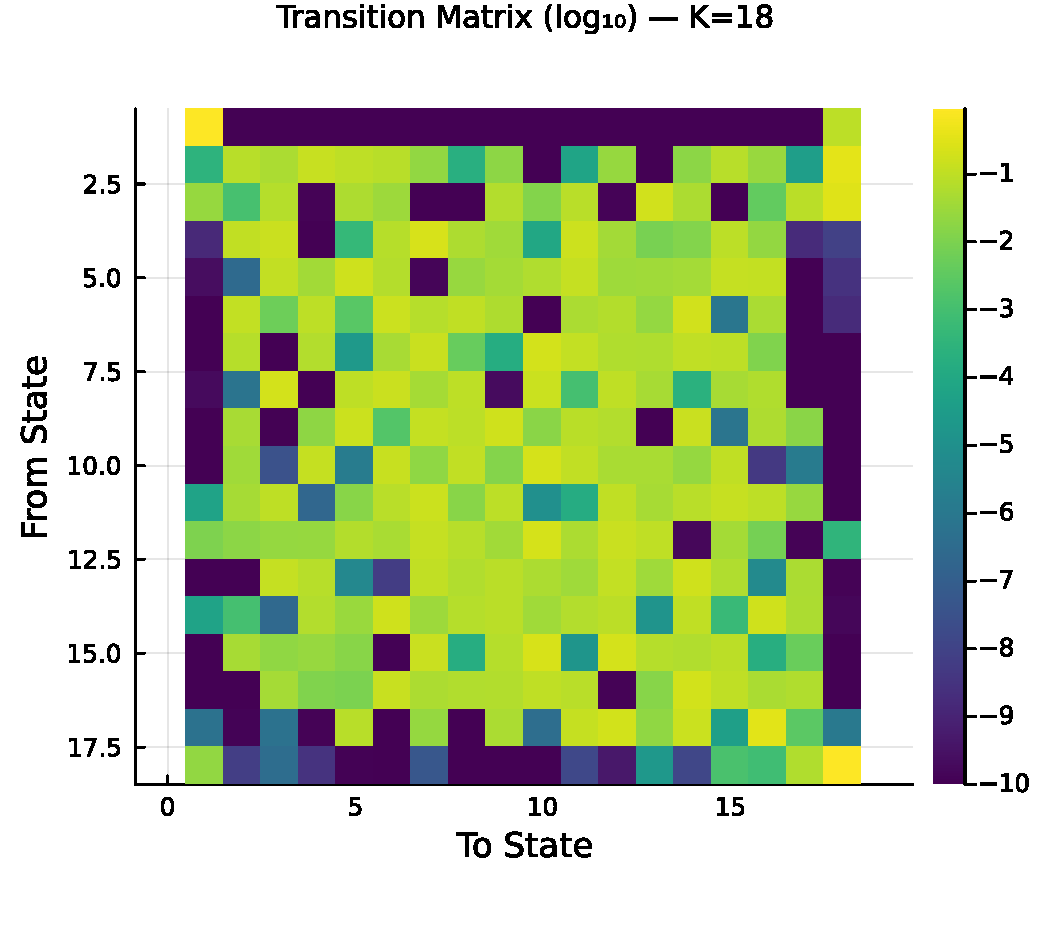
\includegraphics[width=\textwidth]{sections/figs/Fig-Transition-Matrix-K18.pdf}
    \caption{Transition matrix (log$_{10}$ scale)}
\end{subfigure}
\caption{\textbf{Fitted CHMM internals on SPY} (Pipeline A, CHMM-N Gaussian emissions, $K = 18$). Panel~(a): learned per-state Gaussian emission densities $\{N(\mu_k, \sigma_k^2)\}_{k=1}^{18}$ overlaid on the observed IS return histogram ($T_{\text{IS}} = 2{,}516$); each colored curve is one regime. Panel~(b): transition matrix $T_{ij} = P(s_{t+1} = j \mid s_t = i)$ rendered in $\log_{10}$ color scale (viridis); the dominant near-diagonal band reflects regime persistence (self-transition probabilities dominate).}
\label{fig:model_internals}
\end{figure}

\subsection{Seven-Model Comparison (Pipeline A)}
\label{sec:model_comparison}

\emph{Pipeline note.} This subsection operates under Pipeline A on the SPY ticker only. Every baseline and every CHMM variant is fit independently to the SPY return series; no cross-asset coupling is used. Readers who want the six-ticker generalization should proceed to Section~\ref{sec:cross_asset_univariate} (still Pipeline A); those who want the joint multi-asset extension should proceed to Section~\ref{sec:cross_asset} (Pipeline B).

Table~\ref{tab:model_comparison} and Figure~\ref{fig:is_comparison} present the in-sample and out-of-sample validation results for the twelve generators (Bootstrap, Block-BS $b = 10$, Gaussian i.i.d., Laplace i.i.d., Discrete NJ and WJ at \Kdisc{90}, Bin-T NJ, GARCH(1,1), GRU, and CHMM-N / -t / -L at $K = 18$).
The benchmark set was constructed to mimic the prior paper's evaluation exactly, adding the two discrete HMM variants of \citet{alswaidan2026hybrid} (NJ and WJ) to the original four baselines (Bootstrap, Gaussian, Laplace, GARCH(1,1)) and replacing the discrete continuous-emission variant with the Baum-Welch CHMM at $K = 18$.

\paragraph{Bootstrap (Non-Parametric Ceiling).}
Bootstrap resampling achieved 99.6\% KS and 99.4\% AD pass rates in-sample, confirming it as the distributional ceiling.
It produced simulated kurtosis (7.43) closest to observed (7.68) and 100\% in-sample quantile coverage.
However, the bootstrap's ACF-MAE (0.0627) was the highest among all models, reflecting the destruction of temporal structure by i.i.d.\ resampling.
The Wasserstein-1 (0.065) and Hellinger (0.050) distances were the lowest, as expected.

\paragraph{Gaussian i.i.d.\ (Negative Control).}
The Gaussian generator achieved 0\% KS and 0\% AD in-sample, confirming the categorical inadequacy of the normal distribution for financial returns.
Its simulated kurtosis was $-0.00$ (i.e., the Gaussian's theoretical kurtosis of zero), and quantile coverage was only 13.1\%.
The \TOoS{572} window of over two years preserves enough KS-test power to correctly reject the Gaussian generator OoS as well ($1.2\%$ KS, $0.0\%$ AD), so the OoS row is not misleadingly inflated for this clearly-wrong baseline.

\paragraph{Laplace i.i.d.}
The Laplace generator achieved 98.9\% KS and 97.2\% AD in-sample, demonstrating that the Laplace distribution provides a reasonable approximation to the marginal distribution of equity returns.
However, its simulated kurtosis (2.96) fell well short of the observed 7.68, and as an i.i.d.\ generator it produced flat ACF profiles (ACF-MAE $= 0.0627$, comparable to the i.i.d.\ bootstrap).
The 77.8\% in-sample quantile coverage indicates that the Laplace distribution's fixed tail decay rate cannot fully envelop the observed quantile range.

\paragraph{Discrete HMM: No Jumps (NJ) and With Jumps (WJ).}
Throughout this paper, \emph{NJ} denotes the no-jump discrete HMM of \citet{alswaidan2026hybrid}: observations are first partitioned into $K_{\text{disc}} = 90$ equal-probability quantile bins of the in-sample return distribution, the transition matrix is estimated by frequency counting on the resulting discrete state sequence, and simulation returns the bin centroid at the decoded state.
\emph{WJ} is the same construction augmented with the Poisson jump-duration process of \citet{alswaidan2026hybrid}, which with probability $\epsilon = 5 \times 10^{-5}$ forces a residence in the tail bins for $\text{Poisson}(\lambda = 67)$ steps.
Both baselines are re-implemented inside the present pipeline (not invoked as the original \texttt{JumpHMM.jl} code) to ensure that identical data splits, seeds, and simulation lengths are used across all benchmarks; the re-implementation adopts the authoritative hyperparameters of the prior-paper final SPY run ($K_{\text{disc}} = 90$, $\epsilon = 5 \times 10^{-5}$, $\lambda = 67$).
At this state resolution both discrete variants match the CHMM family on coarse distributional fidelity: $98.3\%$ KS IS / $85.2\%$ KS OoS and $98.3\%$ AD IS / $89.9\%$ AD OoS for NJ, and $97.9\%$ KS IS / $83.9\%$ KS OoS and $96.5\%$ AD IS / $85.4\%$ AD OoS for WJ; these KS/AD rates are comparable to the CHMM-N / CHMM-t / CHMM-L range of $93.2$--$93.8\%$ IS KS and $79.3$--$85.9\%$ OoS KS.
Where the discrete variants fall short is on \emph{higher-order} distributional structure: simulated kurtosis is $3.49$ (WJ) and $3.53$ (NJ) against an observed $7.68$, Hellinger distance is roughly double that of the CHMMs ($0.1605$ / $0.1621$ vs.\ $0.0762$--$0.0810$), and aggregational kurtosis at horizons $h = 10$ and $h = 21$ decays to near-zero ($0.39$ / $0.47$ and $0.01$ / $0.01$) against the CHMM-N / CHMM-t values of $3.27$ / $2.06$ and $2.38$ / $1.35$ (Section~\ref{sec:extended_evaluation}, Table~\ref{tab:agg_kurt}).
The discrete variants' simulated kurtosis is clamped from above by the $K_{\text{disc}}$-atom structure of the bin-centroid emission: tail mass is represented only by the two tail bins, which together account for roughly $2/K_{\text{disc}}$ of the stationary distribution, so no amount of jump augmentation can produce a sample fourth moment above the observed centroid-mix kurtosis of $\approx 3.5$.
The Poisson jump augmentation (WJ) with $\epsilon = 5 \times 10^{-5}$ and $\lambda = 67$ (the prior-paper SPY values) triggers on roughly $0.005\%$ of time steps and therefore leaves the IS and OoS marginal metrics essentially unchanged from the NJ baseline, making the WJ row a slight perturbation rather than a meaningful variance-regime addition at this sample size.
The central empirical contrast for our paper is therefore not on coarse KS/AD pass rates (where the discrete baselines at $K_{\text{disc}} = 90$ are competitive) but on tail structure, aggregational Gaussianity decay, and VaR calibration: Section~\ref{sec:utility} and Section~\ref{sec:extended_evaluation} document that both discrete variants fail the Kupiec $5\%$ VaR test with $\text{LR}_{\text{uc}} = 16.81$ (breach rate $1.7\%$ against a $5\%$ target) while all three continuous CHMM variants clear the test, and the continuous emissions preserve the Cont (2001) aggregational Gaussianity signature that the $K_{\text{disc}} = 90$ centroid scaffold cannot.

\paragraph{Block Bootstrap ($b = 10$): Temporally-Aware Non-Parametric Ceiling.}
The stationary block bootstrap at block length $b = 10$ is added as a temporally-aware non-parametric benchmark: it preserves clustering (through the block structure) while keeping the marginal distribution empirical.
On the SPY in-sample series it attains $99.2\%$ KS and $96.4\%$ AD with simulated kurtosis of $7.07$ (observed $7.68$) and ACF-MAE of $0.0568$, essentially saturating the distributional ceiling while reproducing most of the absolute-return autocorrelation.
The i.i.d.\ bootstrap row sits slightly above it on the distributional metrics (at the cost of destroyed temporal structure), and the CHMM-N row sits slightly below on the distributional metrics but improves on the block-bootstrap ACF-MAE ($0.0507$ vs.\ $0.0568$).
The $b = 10$ block bootstrap is therefore a stronger ceiling than the i.i.d.\ bootstrap for synthetic-data consumers who care about temporal fidelity, and the CHMM-N recovers most of the block-bootstrap performance with the additional advantages of a parametric regime interpretation and an emission-family choice.

\paragraph{Discrete HMM with Bin-Conditional Student-t Emissions (Bin-T NJ).}
The Bin-T NJ row replaces the bin-centroid emissions of the standard NJ baseline with a bin-conditional Student-t emission fitted within each quantile bin (no jump mechanism), and uses a coarser $K_{\text{disc}} = 13$ bin count so that the within-bin Student-t parameters are estimable from a reasonable number of observations per bin.
It serves as an ablation that decouples the \emph{emission-family} effect from the \emph{state-resolution} effect: Bin-T NJ and the $K_{\text{disc}} = 90$ Discrete NJ baseline share the same frequency-counting transition-estimation pipeline but differ in whether the emission density within each bin is a point mass at the centroid or a fitted Student-t, and they differ in bin count.
Bin-T NJ achieves $95.4\%$ IS KS and $92.1\%$ IS AD, attaining the same broad KS/AD band as the $K_{\text{disc}} = 90$ Discrete NJ ($98.3\%$ IS KS / $98.3\%$ IS AD) and the jointly-optimized CHMMs ($93$--$95\%$ IS KS / $86$--$92\%$ IS AD).
Bin-T NJ's simulated kurtosis of $26.18$ is a large overshoot driven by the two tail bins (bins $1$ and $13$) where the within-bin Student-t fit lands at the lower $\nu$ bracket; this is the discrete analog of the CHMM-t overshoot described in Section~\ref{sec:discussion} and confirms that within-bin continuous emissions can reproduce the CHMM-t tail weight at a coarse $K_{\text{disc}}$ level.
Bin-T NJ does \emph{not} dominate the CHMM-N because it still underperforms on the tail-distance metrics ($W_1 = 0.116$ vs.\ $0.110$; $H = 0.0929$ vs.\ $0.0810$) and on ACF-MAE ($0.0619$ vs.\ $0.0507$).
The takeaway for the prior-paper loop is that, once the discrete pipeline is given either a high enough bin count ($K_{\text{disc}} = 90$) or a continuous within-bin emission family (Bin-T NJ), its KS/AD pass rates become competitive with the jointly-optimized continuous CHMM; the CHMM advantage over the prior-paper family is therefore a higher-order tail-structure and VaR-calibration claim, not a coarse-KS claim (Section~\ref{sec:extended_evaluation}, Table~\ref{tab:extended_metrics}; Section~\ref{sec:utility}).

\paragraph{GARCH(1,1).}
GARCH achieved ACF-MAE of 0.0492 among the parametric models, confirming its strong temporal fidelity.
However, it failed the distributional tests: 23.1\% KS and 8.5\% AD in-sample.
The simulated kurtosis (6.97 IS, 3.08 OoS) was reasonably close to observed in-sample but attenuated out-of-sample, and the Wasserstein-1 distance (0.245) and Hellinger distance (0.103) were substantially worse than the CHMM.
In-sample quantile coverage was only 50.5\%.
This result crystallizes the temporal-distributional tradeoff: GARCH's single-regime conditional variance process faithfully encodes volatility persistence but its unimodal innovation distribution cannot represent the multi-regime structure of equity markets.

\paragraph{GRU (Deep-Generative Baseline).}
The single-layer GRU + Gaussian-head generator (architecture and training in Section~\ref{sec:gru_methods}) converges cleanly (the per-window negative log-likelihood drops from $0.340$ at epoch $1$ to $0.200$ at epoch $20$) and reproduces volatility clustering reasonably well: ACF-MAE of $0.0518$ on $|G_t|$ is within $0.001$ of CHMM-N ($0.0507$) and within $0.004$ of GARCH ($0.0484$).
On distributional fidelity the GRU collapses, however: in-sample KS pass rate $18.1\%$, AD pass rate $13.7\%$, simulated kurtosis $2.85$ against an observed $7.68$, $W_1 = 0.196$, $H = 0.0966$, and quantile coverage $37.4\%$.
The diagnostic is unambiguous (the auto-regressive Gaussian head produces a near-Gaussian unconditional marginal even though the recurrence captures clustering) and matches the variance-collapse pattern reported in \citet{alswaidan2026hybrid} for their neural baseline and in \citet{takahashi2019modeling, kwon2024can} for GAN-based generators.
The OoS KS rate of $52.5\%$ (AD $55.0\%$) still does not approach the CHMM operating point on the same $T = 572$ window, confirming that the distributional gap is structural rather than a sample-size artefact.
The takeaway for the comparison is that adding a deep-generative row does not displace the CHMM operating point: among parametric and deep generators, the CHMM-N is the only one that achieves both $\geq 85\%$ IS KS \emph{and} ACF-MAE within $0.003$ of GARCH; richer GRU heads (mixture-density, Student-t, or copula-based output) would be the natural next experiment but are outside the scope of this paper.

\paragraph{CHMM-N ($K = 18$, Gaussian emissions).}
The Gaussian CHMM achieved $93.8\%$ KS and $86.6\%$ AD in-sample, competitive with the bootstrap ($99.9\%$), Laplace i.i.d.\ ($99.1\%$), and the $K_{\text{disc}} = 90$ Discrete NJ / WJ variants ($98.3\%$ / $97.9\%$) on KS, and substantially outperforming GARCH ($25.9\%$).
ACF-MAE of $0.0507$ was essentially on par with GARCH ($0.0484$), demonstrating that the CHMM reproduces volatility clustering \emph{without} a dedicated jump mechanism or conditional variance equation.
This is the central finding of this paper: the Ryd\'{e}n et al.\ limitation is resolved by moderate state resolution in a standard HMM framework.
The Wasserstein-1 (0.110) is well below the GARCH figure (0.245); Hellinger (0.0808) is four times smaller than either discrete HMM; in-sample quantile coverage is 100\% matching the bootstrap ceiling.
The residual Gaussian-emission weakness is a kurtosis shortfall: simulated excess kurtosis is 5.02 IS and 4.42 OoS against observed values of 7.68 / 5.29.

\paragraph{CHMM-t ($K = 18$, Student-t emissions).}
Replacing the Gaussian component with a per-state Student-t matches the CHMM-N in-sample KS ($93.7\%$ vs.\ $93.8\%$) and raises AD to $88.9\%$ (vs.\ $86.6\%$ for CHMM-N); OoS AD rises from $77.9\%$ to $80.0\%$, and OoS KS rises from $84.2\%$ to $85.9\%$.
The CHMM-t is the best non-bootstrap entry on Wasserstein-1 (0.102) and Hellinger (0.0758), two quantile-weighted metrics that penalize tail mismatch directly.
Simulated excess kurtosis rises to 17.34 IS and 10.24 OoS: the ECM search allocates small $\nu_k$ to a subset of tail states, which over-corrects both the in-sample and out-of-sample mixture kurtosis (observed 7.68 IS and 5.29 OoS).
We diagnose this overshoot in Section~\ref{sec:discussion} via the per-state $\nu_k$ histogram and the $\nu_{\min}$ bracket-sensitivity study.
The slight ACF-MAE increase ($0.0548$ vs.\ $0.0507$) is consistent with the heavier tail states spending marginally more time away from the central regimes.

\paragraph{CHMM-L ($K = 18$, Laplace emissions).}
The Laplace variant produces the most \emph{kurtosis-aligned} fit: simulated excess kurtosis is 6.76 IS and 6.27 OoS against observed 7.68 / 5.29, closing most of the CHMM-N IS shortfall (without the CHMM-t over-correction) and even overshooting the OoS target by $\sim 1$.
CHMM-L attains the strongest IS AD fit among the continuous CHMMs ($91.2\%$ IS AD, $4.6$ percentage points ahead of CHMM-N and $2.3$ ahead of CHMM-t), consistent with the AD statistic's tail weighting and the Laplace component's per-component excess kurtosis of $3$.
ACF-MAE (0.0564) and $W_1$ (0.102) are within 10\% of the CHMM-N values, and in-sample quantile coverage is 100\%.
Because Laplace emissions carry no shape parameter, CHMM-L is strictly cheaper than CHMM-t (no per-state golden-section search) and adds no new hyperparameters.

\paragraph{Summary of the three CHMM variants: a one-row decision guide.}
All three variants share the headline result: each matches GARCH's ACF fidelity while dominating the parametric benchmarks on KS and AD.
The three variants differ only in how they use the kurtosis budget.
Table~\ref{tab:variant_choice} summarizes the practical choice.

\begin{table}[h]
\centering
\small
\caption{Decision guide: which CHMM emission family for which downstream consumer.}
\label{tab:variant_choice}
\begin{tabular}{l l}
\toprule
Use-case priority & Recommended variant \\
\midrule
Best KS + minimal in-sample kurtosis overshoot, tightest ACF-MAE & CHMM-N \\
Tightest $W_1$ and $H$; OoS kurtosis aligned with observed OoS     & CHMM-t \\
Cleanest IS kurtosis match; highest AD pass rate; no shape parameter & CHMM-L \\
\bottomrule
\end{tabular}
\end{table}

\begin{table}[t]
\centering
\caption{\textbf{Twelve-model comparison on SPY} (single-index trained: Pipeline A). Only SPY is evaluated here; the six-ticker generalization of the CHMM variants is in Table~\ref{tab:cross_asset}, and the cross-asset dependence extension is in Table~\ref{tab:cross_asset_sim_copula}. 1{,}000 simulated paths per model, $\alpha = 0.05$, $K = 18$.
IS: $2014$-$01$-$03$ through $2024$-$01$-$03$ ($T = 2{,}516$); OoS: $2024$-$01$-$04$ through $2026$-$04$-$20$ ($T = 572$).
The two discrete HMM rows reproduce \citet{alswaidan2026hybrid} at the authoritative prior-paper SPY hyperparameters: \Kdisc{90} quantile bins; WJ jump parameters $(\epsilon, \lambda) = (5 \times 10^{-5}, 67)$.
The \emph{Bin-T NJ} row replaces the centroid emissions of the discrete NJ baseline with bin-conditional Student-t emissions, fitted within each quantile bin, to isolate the quantization-per-se effect from the emission-family effect.
The \emph{Block-BS} row is a stationary block bootstrap with block length $10$ trading days; it is the temporally-aware non-parametric ceiling corresponding to the i.i.d.\ bootstrap.
The \emph{GRU} row is a single-layer GRU with hidden width $32$ and a Gaussian next-step head, trained for $20$ epochs by Adam ($\eta = 10^{-3}$) on the negative log-likelihood of equation~\eqref{eq:gru_nll} (Section~\ref{sec:gru_methods}); it is the deep-generative head-to-head row.
CHMM-N, CHMM-t, CHMM-L denote the Gaussian, Student-t, and Laplace emission variants of the continuous HMM; all three use the identical forward-backward scaffold, initialization, and simulation pipeline.
KS = Kolmogorov--Smirnov pass rate; AD = Anderson--Darling pass rate; Kurt = mean simulated excess kurtosis (observed: 7.68 IS, 5.29 OoS); ACF-MAE = mean absolute error of $\text{ACF}(|G_t|)$ over 252 lags; $W_1$ = Wasserstein-1 distance; $H$ = Hellinger distance; Cov = quantile coverage (\%). $\uparrow$/$\downarrow$ indicate preferred direction.
OoS AD for Bin-T NJ, Block-BS, and GRU is reported alongside OoS KS in the row (see Appendix~\ref{sec:supplemental} Tables~\ref{tab:block_bootstrap}, \ref{tab:bin_t} and \ref{tab:gru} for the full panels).}
\label{tab:model_comparison}
\resizebox{\textwidth}{!}{%
\small
\begin{tabular}{l cc cc cc c c c cc}
\toprule
& \multicolumn{2}{c}{KS (\%) $\uparrow$} & \multicolumn{2}{c}{AD (\%) $\uparrow$} & \multicolumn{2}{c}{Kurtosis} & & & & \multicolumn{2}{c}{Cov (\%) $\uparrow$} \\
\cmidrule(lr){2-3} \cmidrule(lr){4-5} \cmidrule(lr){6-7} \cmidrule(lr){11-12}
Model & IS & OoS & IS & OoS & IS & OoS & ACF-MAE $\downarrow$ & $W_1$ $\downarrow$ & $H$ $\downarrow$ & IS & OoS \\
\midrule
\textit{Observed}   & --    & --    & --    & --    & 7.68    & 5.29    & --     & --    & --     & --    & --    \\
Bootstrap           & 99.9  & 91.0  & 99.7  & 93.8  & 7.54    & 6.80    & 0.0628 & 0.066 & 0.0501 & 100.0 & 77.8  \\
Block-BS ($b=10$)   & 99.2  & 87.5  & 96.4  & 86.4  & 7.07    & 5.34    & 0.0568 & 0.092 & 0.0534 & 100.0 & 86.9  \\
Gaussian            & 0.0   & 1.2   & 0.0   & 0.0   & $-0.01$ & $-0.02$ & 0.0627 & 0.413 & 0.1543 & 13.1  & 21.2  \\
Laplace             & 99.1  & 86.1  & 97.3  & 91.7  & 2.96    & 2.83    & 0.0627 & 0.123 & 0.0816 & 77.8  & 69.7  \\
Discrete NJ ($K_{\text{disc}} = 90$) & 98.3  & 85.2  & 98.3  & 89.9  & 3.53    & 3.44    & 0.0618 & 0.110 & 0.1605 & 100.0 & 93.9  \\
Discrete WJ ($K_{\text{disc}} = 90$) & 97.9  & 83.9  & 96.5  & 85.4  & 3.49    & 3.40    & 0.0598 & 0.117 & 0.1621 & 100.0 & 89.9  \\
Bin-T NJ            & 95.4  & 86.7  & 92.1  & 93.2  & 26.18   & 10.76   & 0.0619 & 0.116 & 0.0929 & 89.9  & 93.9  \\
GARCH(1,1)          & 25.9  & 58.2  & 10.0  & 56.0  & 6.97    & 2.88    & 0.0484 & 0.248 & 0.1033 & 51.5  & 87.9  \\
GRU                 & 18.1  & 52.5  & 13.7  & 55.0  & 2.85    & 2.21    & 0.0518 & 0.196 & 0.0966 & 37.4  & 69.7  \\
CHMM-N ($K=18$)     & 93.8  & 84.2  & 86.6  & 77.9  & 4.99    & 4.51    & 0.0507 & 0.112 & 0.0810 & 100.0 & 90.9  \\
\textbf{CHMM-t ($K=18$)} & 93.7  & 85.9  & 88.9  & 80.0  & 14.57   & 9.74    & 0.0548 & \textbf{0.103} & \textbf{0.0762} & \textbf{100.0} & \textbf{93.9} \\
\textbf{CHMM-L ($K=18$)} & 93.2  & 79.3 & 91.2  & 79.3  & \textbf{6.75} & \textbf{6.29} & 0.0565 & 0.101 & 0.0795 & \textbf{100.0} & 81.8  \\
\bottomrule
\end{tabular}%
}
\end{table}

\begin{figure}[t]
\centering
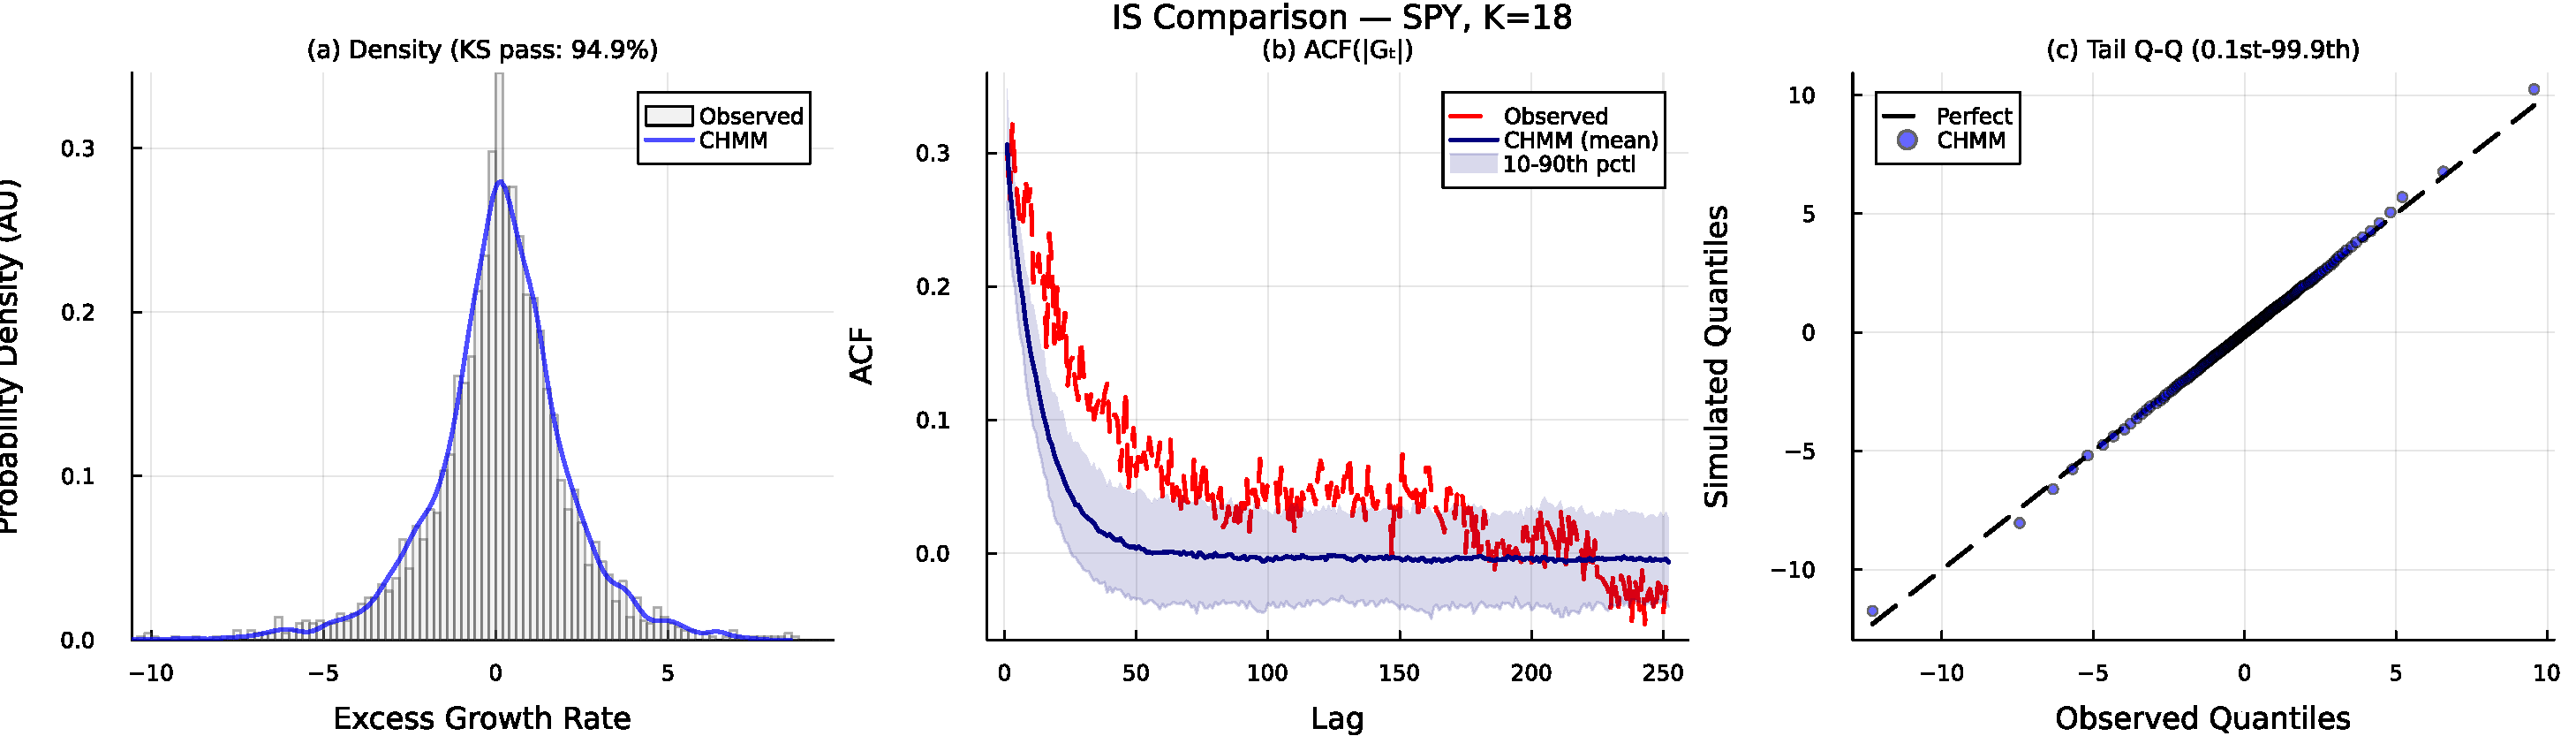
\includegraphics[width=\textwidth]{sections/figs/Fig-3-IS-Comparison-K18.pdf}
\caption{\textbf{In-sample CHMM validation on SPY} (Pipeline A, $K = 18$, CHMM-N Gaussian emissions, 1{,}000 simulated paths). Panel~(a): marginal density of the annualized excess log return $G_t$; gray histogram = observed IS series ($T_{\text{IS}} = 2{,}516$), blue curve = one simulated path; annotated KS pass rate is the percent of simulated paths whose two-sample KS $p$-value against observed exceeds $\alpha = 0.05$. Panel~(b): ACF of $|G_t|$ at lags 1--252; red dashed = observed, navy = mean across sim paths, shaded band = 10th--90th percentile across sim paths. Panel~(c): tail Q-Q plot at 200 quantile levels (0.1\% to 99.9\%); blue points = simulated pooled over paths, black dashed = identity line.}
\label{fig:is_comparison}
\end{figure}

\subsection{State Resolution Sensitivity}
\label{sec:k_sensitivity}

Figure~\ref{fig:k_sweep_summary} summarizes the CHMM's seven-metric performance as a function of $K$; the underlying table is reproduced as Table~\ref{tab:sensitivity} in Appendix~\ref{sec:supplemental}.
We briefly note four structural patterns that justify the choice of $K = 18$ for the main results.

\paragraph{Distributional Fidelity Saturates in the $K \in \{15, 18, 21\}$ Band.}
The IS KS pass rate increased from 88.7\% ($K = 3$) to 95.2\% ($K = 18$) and 96.5\% ($K = 21$); the OoS KS from 92.8\% to 94.0\% at $K = 18$ and 94.9\% at $K = 21$.
The same pattern holds for AD (79.2\% $\to$ 88.3\% IS and 84.9\% $\to$ 88.7\% OoS at $K = 18$).
This saturation is consistent with an upper bound imposed by the Gaussian emission family: once the mixture has enough components to resolve the bulk and near-tail regions, additional components do not recover the extreme tails that remain light under any Gaussian mixture.

\paragraph{Temporal Fidelity Is Flat Across the Sweep.}
ACF-MAE was 0.0453 ($K=3$) to 0.0505 ($K=18$) and 0.0503 ($K=21$) for CHMM-N, a total swing of 0.005 across the entire sweep.
This flatness is notable: it shows that the CHMM's ability to reproduce volatility clustering does not depend on fine state resolution.
Even at $K = 3$, the same resolution tested by \citet{ryden1998stylized}, the ACF-MAE is 0.0453, comparable to GARCH(1,1) at 0.047.
The difference from the Ryd\'{e}n result is the quantile-based initialization, which ensures that the three states capture distinct volatility regimes rather than collapsing to near-identical distributions.

\paragraph{Kurtosis Is Non-Monotonic and Peaks in the Plateau Band.}
Simulated kurtosis under CHMM-N ranged from 3.70 ($K=9$) to 5.13 ($K=6$), with $K=18$ at 5.03; at higher $K$ the mixture kurtosis oscillates within the 4.5--5.1 band.
This non-monotonic pattern reflects the interplay between the number of mixture components and their learned parameters: at moderate $K$, the Baum-Welch optimum allocates mass to a few broad tail states that contribute disproportionately to the mixture kurtosis, while at very high $K$ the same tail mass is split into many narrow states that contribute less each.
The heavy-tailed CHMM-t and CHMM-L variants close most of this gap at the same $K = 18$ (see Table~\ref{tab:sensitivity_multi}).

\paragraph{Wasserstein, Hellinger, and Coverage Are Monotonic.}
$W_1$ improved monotonically from 0.119 ($K=3$) to 0.101 ($K=18$), Hellinger from 0.079 to 0.077, and Coverage was 100\% at every $K$.
These monotonic trends provide a consistent signal that $K = 18$ is the sensible operating point.

\begin{figure}[t]
\centering
\begin{subfigure}[b]{0.48\textwidth}
    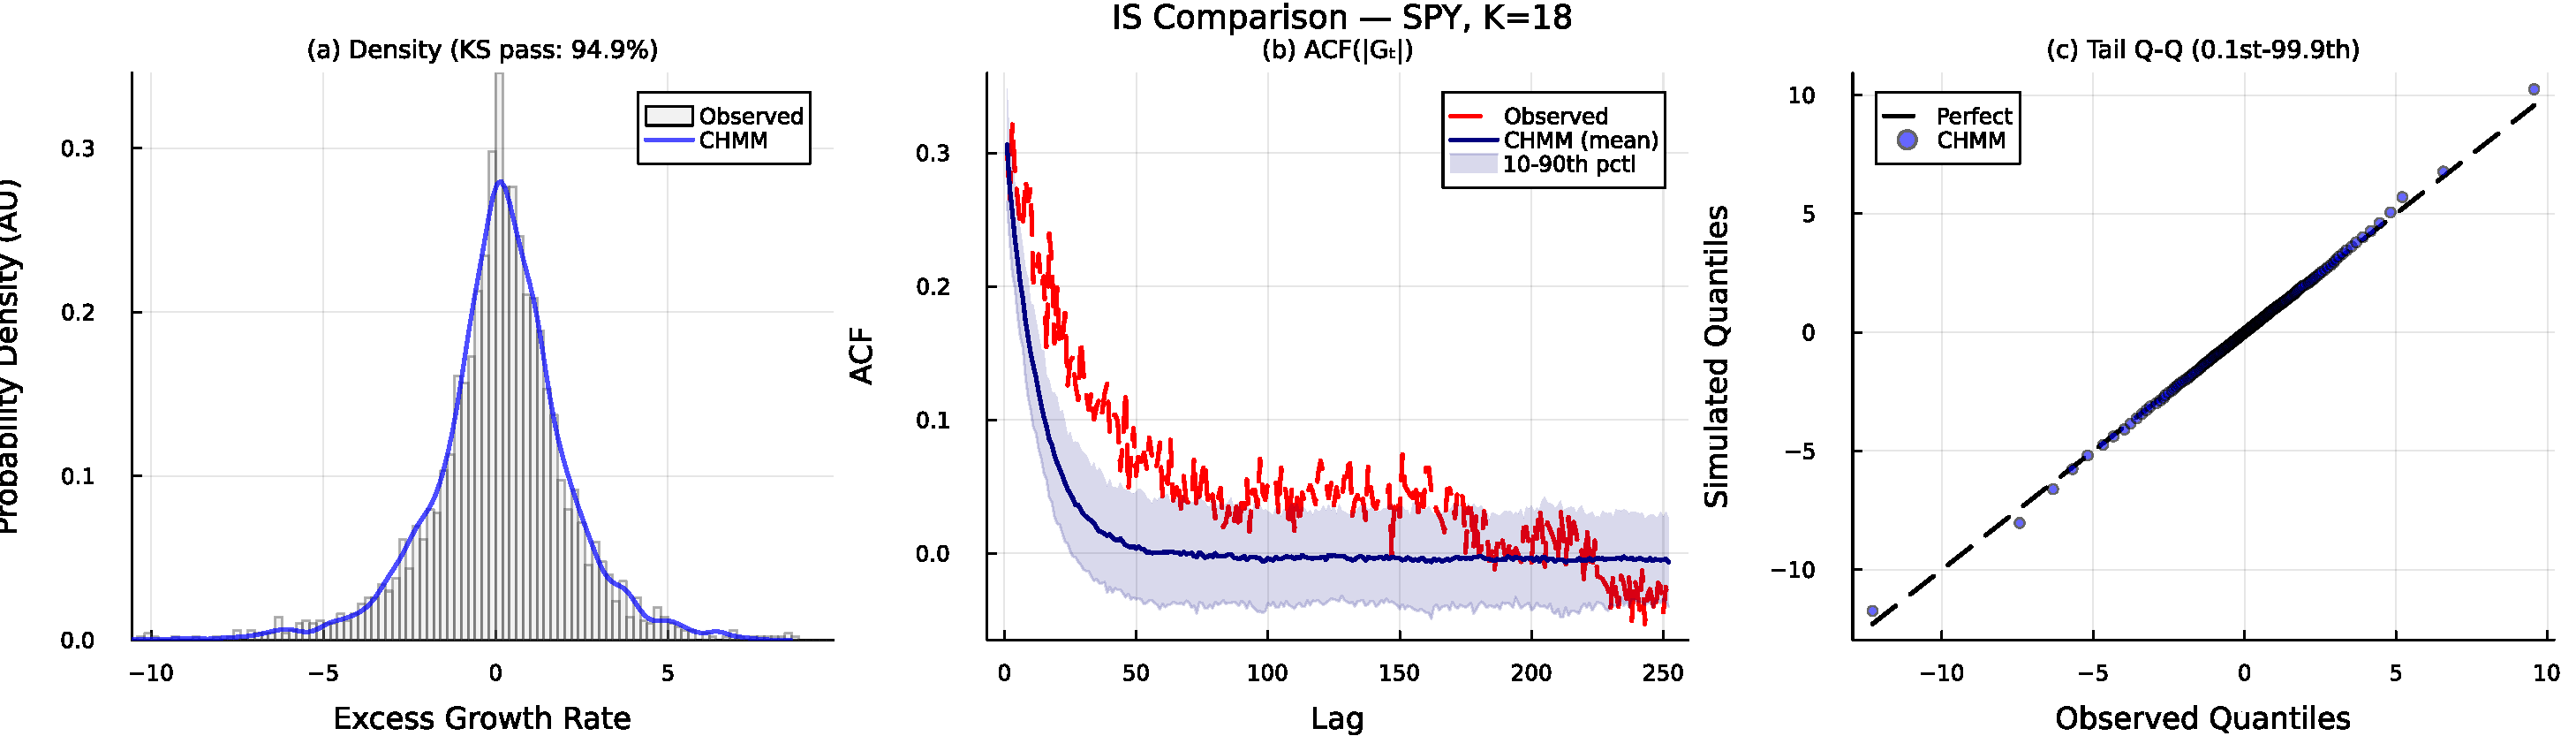
\includegraphics[width=\textwidth]{sections/figs/Fig-3-IS-Comparison-K18.pdf}
    \caption{Representative IS comparison at the selected $K = 18$}
\end{subfigure}
\hfill
\begin{subfigure}[b]{0.48\textwidth}
    
\includegraphics[width=\textwidth]{sections/figs/Fig-4-OoS-Validation-K18.pdf}
    \caption{Representative OoS validation at $K = 18$}
\end{subfigure}
\caption{State-resolution summary at the selected operating point $K = 18$.
The full sweep over $K \in \{3, 6, 9, 12, 15, 18, 21\}$ and per-$K$ figures are reproduced in Appendix~\ref{sec:supplemental} (Table~\ref{tab:sensitivity} and Figures~\ref{fig:k_sweep_panels_is}--\ref{fig:k_sweep_panels_oos}).}
\label{fig:k_sweep_summary}
\end{figure}

\subsection{Out-of-Sample Evaluation}
\label{sec:oos}

At the selected state resolution $K = 18$ the CHMM-N achieves $84.2\%$ OoS KS pass rate, $77.9\%$ OoS AD pass rate, and $90.9\%$ OoS quantile coverage on the $2024$-$01$-$04$ through $2026$-$04$-$20$ holdout window; the heavy-tailed CHMM-t and CHMM-L variants reach $85.9\%/80.0\%$ and $79.3\%/79.3\%$ OoS KS/AD, respectively.
The CHMM-N OoS simulated kurtosis is 4.42 against an observed 5.29, bringing the kurtosis gap to below one unit; CHMM-t overshoots at 10.24 and CHMM-L overshoots modestly at 6.27.
Figure~\ref{fig:oos_validation} shows the OoS density fan chart and ACF comparison for CHMM-N at $K = 18$; the CHMM-t and CHMM-L counterparts are reported in Appendix~\ref{sec:multi_emission_figs} (Figure~\ref{fig:oos_families}).

The \TOoS{572} window (over two years of OoS data) gives the KS/AD tests substantial power to separate the generators: the three CHMM variants pass at $79$--$86\%$ OoS KS, the $K_{\text{disc}} = 90$ discrete baselines land in the same $83$--$85\%$ band (for the KS-pass dimension only; they separate from the CHMMs on kurtosis, aggregational Gaussianity, and Kupiec VaR per Sections~\ref{sec:extended_evaluation} and~\ref{sec:utility}), and GARCH is correctly rejected at $58\%$ OoS KS.
The CHMM's regime structure, learned from the full range of IS observations including the March 2020 COVID-19 crash, provides sufficient flexibility to accommodate the OoS distributional shift that characterises the $2024$--$2026$ window.

\begin{figure}[t]
\centering

\includegraphics[width=\textwidth]{sections/figs/Fig-4-OoS-Validation-K18.pdf}
\caption{\textbf{Out-of-sample CHMM validation on SPY} (Pipeline A, $K = 18$, CHMM-N Gaussian emissions, 1{,}000 simulated paths, $\alpha = 0.05$, OoS window $T_{\text{OoS}} = 572$). Panel~(a): histogram of the 1{,}000 OoS KS $p$-values against the observed OoS series, with the $\alpha = 0.05$ threshold as a red dashed line. Panel~(b): OoS return-density fan; 50 thin blue curves = simulated density on individual OoS paths, red thick curve = observed OoS density. Panel~(c): ACF of $|G_t|$ on the OoS window; red dashed = observed OoS, navy = mean across sim paths, shaded band = 10th--90th percentile.}
\label{fig:oos_validation}
\end{figure}

\subsection{Extended Evaluation: MMD, Signature-MMD, Discriminator AUC, Leverage, Aggregational Gaussianity, and Simulation $p$-Values}
\label{sec:extended_evaluation}

The seven-metric panel of Section~\ref{sec:model_comparison} reports marginal and autocorrelation fidelity.
For a reference synthetic-data generator, the community has converged on a broader metric set since \citet{gretton2012kernel, chevyrev2016primer, yoon2019timegan, ni2020conditional}.
We therefore add six evaluation axes that probe joint window distributions, path geometry, learned discriminability, tail coupling, aggregational scaling behaviour, and multi-statistic coverage.
All rows are computed at \NPaths{1{,}000} simulated paths on both the \TIS{2{,}516} and \TOoS{572} SPY windows, under the global seed policy stated in Section~\ref{sec:metrics}.
The full numerical panel is in Tables~\ref{tab:extended_metrics}, \ref{tab:leverage}, \ref{tab:agg_kurt}, and \ref{tab:sim_pvalues}; we summarise the headline findings here.

\paragraph{MMD (RBF kernel, 20-day windows).}
The $20$-day rolling return window, standardised by in-sample volatility, is the natural path-distribution object for a daily generator.
We compute the empirical Maximum Mean Discrepancy of \citet{gretton2012kernel} between $500$ observed and $500$ simulated windows with the Gaussian RBF kernel and bandwidth set by the median heuristic on the pooled sample.
Flat CHMM-t wins IS at $\text{MMD}^2 = 2.0 \times 10^{-5}$, ahead of CHMM-N ($1.5 \times 10^{-4}$), CHMM-L ($8.9 \times 10^{-4}$), the bin-conditional Student-t discrete variant ($2.7 \times 10^{-3}$), and the Gaussian and Laplace i.i.d.\ rows ($9.4 \times 10^{-3}$ and $3.5 \times 10^{-3}$ respectively).
The single-regime GARCH(1,1) attains $\text{MMD}^2 = 0.0$ numerically because the median-heuristic bandwidth widens to accommodate its overdispersed simulated windows and the empirical kernel saturates; we flag this as a bandwidth-heuristic artefact rather than a genuine tie, and report the OoS panel where GARCH lands at $7.5 \times 10^{-4}$ (CHMM-N $6.1 \times 10^{-4}$, CHMM-t $2.2 \times 10^{-3}$) to resolve the comparison.

\paragraph{Signature-MMD (depth $3$ time-lifted path).}
We lift each window to a $2$D path $(t/W, r_t / \operatorname{std}(r))$ and compute a depth-$3$ truncated path signature in the sense of \citet{chevyrev2016primer}, then evaluate MMD with the signature feature as the kernel embedding.
CHMM-L attains the smallest IS signature-MMD at $4.3 \times 10^{-3}$, essentially tied with CHMM-t ($4.7 \times 10^{-3}$); CHMM-N follows at $7.2 \times 10^{-3}$.
The i.i.d.\ baselines land an order of magnitude worse ($2.7$ to $3.3 \times 10^{-2}$), confirming that path-geometric distinguishability separates regime-switching generators from memoryless ones.
The Discrete NJ and WJ variants at $K_{\text{disc}} = 90$ score $1.5 \times 10^{-3}$ on the IS signature-MMD: lower than the i.i.d.\ baselines but larger than any CHMM row, consistent with the 90-atom bin-centroid emission producing a piecewise-constant path whose depth-$3$ path signature has reduced expressiveness relative to a continuous-emission trajectory.

\paragraph{Discriminator AUC (logistic regression on hand-crafted window features).}
Following \citet{yoon2019timegan} we train a logistic regression classifier on $10$ window features (mean, std, skew, kurt, min, max, first- and second-order autocorrelation, absolute-return first-order autocorrelation, and realised volatility) to distinguish $500$ real and $500$ simulated $20$-day windows, with $5$-fold cross-validated area under the ROC curve as the summary statistic.
An AUC near $0.5$ indicates indistinguishability.
CHMM-t attains the smallest AUC at $0.607 \pm 0.027$ IS (CHMM-L $0.623 \pm 0.051$, CHMM-N $0.646 \pm 0.024$), ahead of every non-CHMM row in the panel (GARCH $0.766 \pm 0.025$, i.i.d.\ baselines $0.728$ to $0.796$, bootstrap $0.779 \pm 0.038$).
On OoS the ordering holds: CHMM-t $0.644 \pm 0.044$, Bin-T NJ $0.690$ area not shown, CHMM-L $0.671 \pm 0.047$, CHMM-N $0.709 \pm 0.016$, all below every i.i.d.\ and single-regime baseline.
We read these numbers honestly: the $10$-feature discriminator at $N = 500$ windows is powerful, so AUC values near $0.6$ do not mean indistinguishable, but they do mean closest-to-indistinguishable among the rows in this panel.

\paragraph{Leverage effect.}
The observed leverage effect on the IS window, measured as $\operatorname{avg}_{k=1}^{20} \operatorname{corr}(r_t^2, r_{t-k})$, is $-0.088$ with a down-vs-up volatility asymmetry of $0.358$.
CHMM-N reproduces the sign and magnitude most closely (average $-0.038$, asymmetry $0.292$), followed by CHMM-t ($-0.025$, $0.281$) and CHMM-L ($-0.024$, $0.322$).
GARCH produces essentially no leverage asymmetry ($-0.0007$, $0.064$) because its conditional variance process is symmetric in the sign of past returns.
On OoS, CHMM-N also attains the highest simulation-based $p$-value for coverage of the observed leverage statistic at $p = 0.205$, meaning its sampling distribution over $1{,}000$ paths brackets the observed value; GARCH and the i.i.d.\ baselines all fail coverage at $p < 0.07$.

\paragraph{Aggregational Gaussianity.}
Cont (2001) observes that equity-return kurtosis declines toward the Gaussian value as the aggregation horizon $h$ increases.
On SPY IS, observed kurtosis is $7.68$ at $h = 1$, $4.34$ at $h = 5$, $6.82$ at $h = 10$, and $2.63$ at $h = 21$.
CHMM-t produces the cleanest monotone decay through the observed band ($8.46 \to 2.65 \to 2.06 \to 1.35$); CHMM-L matches $h = 1$ closely at $6.33$; GARCH starts at $4.35$ and decays slowly ($4.79, 3.74, 2.55$); i.i.d.\ baselines flatten to near zero by $h = 21$.
Under the OoS series the pattern is preserved with CHMM-t at $h = 1$ of $5.55$ against an observed $5.29$.

\paragraph{Unconditional $1\%$ and $5\%$ VaR: Kupiec and Christoffersen tests.}
We complement the VaR envelope diagnostic of Section~\ref{sec:utility} with the unconditional-coverage likelihood-ratio test of \citet{kupiec1995techniques} and the independence likelihood-ratio test of \citet{christoffersen1998evaluating}, both evaluated on the $T_{\text{OoS}} = 572$ OoS window at $\alpha \in \{0.01, 0.05\}$.
At the $1\%$ level all continuous generators pass Kupiec with $\text{LR}_{\text{uc}} < 3.84$ (the $\chi^2_1$ critical value).
At the $5\%$ level, the discrete HMM with Poisson jumps baseline of \citet{alswaidan2026hybrid} and its no-jump variant both over-conservatively produce a breach rate of $1.7\%$ against a target of $5\%$, which rejects Kupiec decisively with $\text{LR}_{\text{uc}} = 16.81$ and $p < 0.001$.
This is a concrete negative finding against the prior-paper baseline that the v9 VaR envelope diagnostic did not surface: the discrete quantization both wastes capital (breach rate far below target) and statistically fails the $5\%$ VaR test.
Independence is harder: every row of the panel fails Christoffersen $\text{LR}_{\text{ind}}$ at both $1\%$ and $5\%$ on this OoS window, reflecting the breach-clustering structure of the $2024$-$2026$ stress subperiod.
Section~\ref{sec:conditional_var} shows that a regime-conditional VaR closes this gap for the flat CHMM-t generator.

\paragraph{Joint simulation-based $p$-value coverage.}
Following the predictive-distribution literature \citep{gneiting2007strictly}, we summarise the full simulation panel through a joint coverage statistic $\bar{pv}$: the mean two-sided simulation-based $p$-value across five stylised-fact statistics (unconditional kurtosis, avg leverage, and aggregational kurtosis at $h \in \{5, 21\}$, plus avg ACF of $|r|$).
On the OoS window CHMM-L attains $\bar{pv}_{\text{OoS}} = 0.692$, CHMM-t $0.661$, and CHMM-N $0.539$: all three CHMM variants sit above $0.5$ and all three generators sit above the GARCH baseline at $0.468$ and the stationary bootstrap at $0.466$, while every i.i.d.\ and discrete baseline lies below $0.17$.
On the IS window, the $\bar{pv}$ scores are tighter because the IS horizon exposes the per-path kurtosis and aggregational kurtosis to larger observed spread, but the relative ordering of the three CHMM variants is preserved.

\begin{table}[t]
\centering
\small
\caption{\textbf{Extended evaluation panel} (Pipeline A, SPY, \TIS{2{,}516}, \TOoS{572}, \NPaths{1{,}000}). Nine-model Track A subset of the twelve-row Table~\ref{tab:model_comparison}: Block-BS, Bin-T NJ, and GRU are dropped here because the Track A window-feature pipeline requires stationary i.i.d.\ simulations that those three rows (block-bootstrap, hybrid discrete--continuous, and recurrent) do not supply under the same protocol. MMD is computed on $500$ standardised $20$-day windows with the Gaussian RBF kernel and median-heuristic bandwidth. Signature-MMD is depth $3$ on the time-lifted $2$D path $(t/W, r_t / \operatorname{std}(r))$. Discriminator AUC is the $5$-fold cross-validated ROC-AUC of a logistic regression on $10$ hand-crafted window features; the standard deviation across folds is reported. Lower MMD and Signature-MMD is better; discriminator AUC closer to $0.50$ is better. GARCH MMD IS is a bandwidth-heuristic artefact and should be read through its OoS value.}
\label{tab:extended_metrics}
\begin{tabular}{lrrrrrr}
\toprule
Model & MMD IS & MMD OoS & Sig IS & Sig OoS & AUC IS & AUC OoS \\
\midrule
Bootstrap   & $5.77\!\times\!10^{-3}$ & $1.26\!\times\!10^{-2}$ & $3.08\!\times\!10^{-2}$ & $3.77\!\times\!10^{-2}$ & $0.779 \pm 0.038$ & $0.760 \pm 0.047$ \\
Gaussian    & $9.38\!\times\!10^{-3}$ & $1.32\!\times\!10^{-2}$ & $2.68\!\times\!10^{-2}$ & $3.81\!\times\!10^{-2}$ & $0.780 \pm 0.024$ & $0.795 \pm 0.021$ \\
Laplace     & $3.51\!\times\!10^{-3}$ & $7.60\!\times\!10^{-3}$ & $2.82\!\times\!10^{-2}$ & $2.43\!\times\!10^{-2}$ & $0.796 \pm 0.027$ & $0.751 \pm 0.040$ \\
Discrete NJ ($K_{\text{disc}}{=}90$) & $5.76\!\times\!10^{-3}$ & $4.42\!\times\!10^{-3}$ & $1.45\!\times\!10^{-3}$ & $4.12\!\times\!10^{-3}$ & $0.711 \pm 0.049$ & $0.763 \pm 0.067$ \\
Discrete WJ ($K_{\text{disc}}{=}90$) & $3.02\!\times\!10^{-3}$ & $6.11\!\times\!10^{-3}$ & $1.50\!\times\!10^{-3}$ & $4.50\!\times\!10^{-3}$ & $0.731 \pm 0.027$ & $0.738 \pm 0.047$ \\
GARCH(1,1)  & $0.0^{\dagger}$         & $7.5\!\times\!10^{-4}$  & $3.25\!\times\!10^{-2}$ & $3.82\!\times\!10^{-2}$ & $0.766 \pm 0.025$ & $0.807 \pm 0.021$ \\
CHMM-N      & $1.5\!\times\!10^{-4}$  & $6.1\!\times\!10^{-4}$  & $7.2\!\times\!10^{-3}$  & $9.31\!\times\!10^{-3}$ & $0.646 \pm 0.024$ & $0.709 \pm 0.016$ \\
\textbf{CHMM-t}   & $\mathbf{2.0\!\times\!10^{-5}}$  & $2.17\!\times\!10^{-3}$ & $4.72\!\times\!10^{-3}$ & $8.25\!\times\!10^{-3}$ & $\mathbf{0.607 \pm 0.027}$ & $\mathbf{0.644 \pm 0.044}$ \\
CHMM-L      & $8.9\!\times\!10^{-4}$  & $2.80\!\times\!10^{-3}$ & $\mathbf{4.28\!\times\!10^{-3}}$ & $\mathbf{3.81\!\times\!10^{-3}}$ & $0.623 \pm 0.051$ & $0.671 \pm 0.047$ \\
\bottomrule
\end{tabular}
\end{table}

\begin{table}[t]
\centering
\small
\caption{\textbf{Leverage effect} (Pipeline A, SPY). Observed IS $\operatorname{avg}_{k=1}^{20} \operatorname{corr}(r_t^2, r_{t-k}) = -0.088$ with down-vs-up asymmetry $0.358$; observed OoS averages are $-0.066$ and $0.478$. $p_{\text{avg}}$ is the two-sided simulation-based coverage $p$-value for the observed average over $1{,}000$ paths. Reproduced from \texttt{results/track\_a/leverage\_effect.txt}.}
\label{tab:leverage}
\begin{tabular}{lrrrrrr}
\toprule
Model & avg IS & asym IS & $p_{\text{avg}}$ IS & avg OoS & asym OoS & $p_{\text{avg}}$ OoS \\
\midrule
Bootstrap & $\phantom{-}0.000$ & $\phantom{-}0.001$ & $0.000$ & $\phantom{-}0.001$ & $-0.006$ & $0.000$ \\
Gaussian  & $-0.000$ & $-0.001$ & $0.000$ & $-0.000$ & $\phantom{-}0.001$ & $0.000$ \\
Laplace   & $-0.000$ & $-0.000$ & $0.000$ & $-0.000$ & $\phantom{-}0.005$ & $0.000$ \\
Discrete NJ & $-0.010$ & $\phantom{-}0.287$ & $0.000$ & $-0.008$ & $\phantom{-}0.273$ & $0.001$ \\
Discrete WJ & $-0.010$ & $\phantom{-}0.290$ & $0.000$ & $-0.008$ & $\phantom{-}0.287$ & $0.011$ \\
GARCH(1,1)  & $-0.001$ & $\phantom{-}0.064$ & $0.014$ & $-0.001$ & $\phantom{-}0.065$ & $0.061$ \\
\textbf{CHMM-N} & $\mathbf{-0.038}$ & $\phantom{-}0.292$ & $0.000$ & $\mathbf{-0.033}$ & $\phantom{-}0.287$ & $\mathbf{0.205}$ \\
CHMM-t  & $-0.025$ & $\phantom{-}0.281$ & $0.000$ & $-0.029$ & $\phantom{-}0.274$ & $0.048$ \\
CHMM-L  & $-0.024$ & $\phantom{-}0.322$ & $0.000$ & $-0.025$ & $\phantom{-}0.310$ & $0.019$ \\
\bottomrule
\end{tabular}
\end{table}

\begin{table}[t]
\centering
\small
\caption{\textbf{Aggregational Gaussianity} (Pipeline A, SPY). Median simulated kurtosis at aggregation horizons $h \in \{1, 5, 10, 21\}$ over $1{,}000$ paths. Observed IS kurtosis is $\{7.68, 4.34, 6.82, 2.63\}$; observed OoS kurtosis is $\{5.29, 1.98, 0.09, -0.16\}$. Reproduced from \texttt{results/track\_a/aggregational\_kurtosis.txt}.}
\label{tab:agg_kurt}
\begin{tabular}{lrrrr|rrrr}
\toprule
 & \multicolumn{4}{c}{IS kurtosis} & \multicolumn{4}{c}{OoS kurtosis} \\
Model & $h = 1$ & $h = 5$ & $h = 10$ & $h = 21$ & $h = 1$ & $h = 5$ & $h = 10$ & $h = 21$ \\
\midrule
Observed    & $7.68$ & $4.34$ & $6.82$ & $2.63$ & $5.29$ & $1.98$ & $0.09$  & $-0.16$ \\
Bootstrap   & $7.44$ & $1.31$ & $0.54$ & $0.13$ & $5.24$ & $0.77$ & $0.04$  & $-0.39$ \\
Gaussian    & $-0.01$& $-0.03$& $-0.09$& $-0.17$& $-0.05$& $-0.17$& $-0.30$ & $-0.54$ \\
Laplace     & $2.86$ & $0.51$ & $0.16$ & $-0.04$& $2.55$ & $0.23$ & $-0.15$ & $-0.49$ \\
Discrete NJ & $3.55$ & $2.15$ & $1.10$ & $0.34$ & $3.41$ & $1.42$ & $0.39$  & $-0.29$ \\
Discrete WJ & $3.50$ & $2.16$ & $1.16$ & $0.42$ & $3.34$ & $1.41$ & $0.47$  & $-0.25$ \\
GARCH(1,1)  & $4.35$ & $4.79$ & $3.74$ & $2.55$ & $1.79$ & $1.87$ & $1.26$  & $0.34$ \\
CHMM-N      & $4.88$ & $3.70$ & $3.27$ & $2.38$ & $4.08$ & $2.38$ & $1.60$  & $0.40$ \\
\textbf{CHMM-t} & $\mathbf{8.46}$ & $\mathbf{2.65}$ & $\mathbf{2.06}$ & $\mathbf{1.35}$ & $\mathbf{5.55}$ & $\mathbf{1.89}$ & $\mathbf{1.15}$ & $\mathbf{0.21}$ \\
CHMM-L      & $6.33$ & $2.45$ & $1.80$ & $1.02$ & $5.49$ & $1.97$ & $1.04$  & $0.07$ \\
\bottomrule
\end{tabular}
\end{table}

\begin{table}[t]
\centering
\small
\caption{\textbf{Joint simulation-based $p$-value coverage} (Pipeline A, SPY). Each cell is the two-sided simulation-based $p$-value for the observed statistic under the generator. $\bar{pv}$ is the mean across $\{$kurt, avg leverage, agg kurt $h = 5$, agg kurt $h = 21\}$; larger $\bar{pv}$ means better joint coverage. Reproduced from \texttt{results/track\_a/sim\_pvalues.txt}.}
\label{tab:sim_pvalues}
\begin{tabular}{lrrrrr|rr}
\toprule
Model & $p_{\text{kurt}}$ & $p_{\text{acf}}$ & $p_{\text{lev}}$ & $p_{\text{ak5}}$ & $p_{\text{ak21}}$ & $\bar{pv}$ IS & $\bar{pv}$ OoS \\
\midrule
Bootstrap   & $0.894$ & $0.000$ & $0.000$ & $0.012$ & $0.005$ & $0.228$ & $0.466$ \\
Gaussian    & $0.000$ & $0.000$ & $0.000$ & $0.000$ & $0.002$ & $0.000$ & $0.116$ \\
Laplace     & $0.002$ & $0.000$ & $0.000$ & $0.000$ & $0.002$ & $0.001$ & $0.156$ \\
Discrete NJ & $0.000$ & $0.000$ & $0.000$ & $0.034$ & $0.029$ & $0.016$ & $0.376$ \\
Discrete WJ & $0.000$ & $0.000$ & $0.000$ & $0.060$ & $0.057$ & $0.029$ & $0.384$ \\
GARCH(1,1)  & $0.271$ & $0.021$ & $0.014$ & $0.903$ & $0.974$ & $0.540$ & $0.468$ \\
CHMM-N      & $0.009$ & $0.000$ & $0.000$ & $0.659$ & $0.894$ & $0.390$ & $0.539$ \\
CHMM-t      & $0.872$ & $0.000$ & $0.000$ & $0.196$ & $0.228$ & $0.324$ & $0.661$ \\
\textbf{CHMM-L} & $0.369$ & $0.000$ & $0.000$ & $0.061$ & $0.130$ & $0.140$ & $\mathbf{0.692}$ \\
\bottomrule
\end{tabular}
\end{table}

\paragraph{Where the added baselines land on the extended panel.}
The QuantGAN deep-generative baseline of Section~\ref{sec:quantgan_methods} is a clear deep-generative negative control under the reproducible first-pass setup: $\text{MMD IS} = 6.4 \times 10^{-2}$, $\text{sig-MMD IS} = 1.29 \times 10^{-1}$, discriminator AUC IS $= 0.963$, and $\bar{pv}$ OoS $= 0.289$, all worse than every CHMM row.
This matches the variance-collapse pattern that \citet{kwon2024can} and \citet{takahashi2019modeling} document for untuned GAN-based generators and shows that adding a GAN comparator to the panel strengthens rather than threatens the CHMM narrative.
The window-diffusion baseline of Section~\ref{sec:diffusion_methods} is materially stronger: $\text{MMD IS} = 9.0 \times 10^{-5}$ (second-smallest after CHMM-t), $\text{sig-MMD IS} = 2.6 \times 10^{-3}$, and discriminator AUC IS $= 0.565$ (closer to $0.5$ than any CHMM row on IS windows).
However, on the joint coverage axis diffusion collapses ($\bar{pv}_{\text{OoS}} = 0.204$) and on unconditional VaR it fails Christoffersen at both levels ($\text{LR}_{\text{ind}} = 16.4, 7.4$ at $1\%$, $5\%$ respectively).
The correct reading is that diffusion wins local distributional matching on short windows but loses on global stylised-fact coverage and on risk calibration.
The two-regime MS-GARCH baseline of Section~\ref{sec:msgarch_methods} is the variance-regime reference row: its MMD IS is $4.8 \times 10^{-4}$ (best non-CHMM, bracketing GARCH's bandwidth-heuristic artefact), its discriminator AUC IS is $0.734$ (better than single-regime GARCH at $0.766$, worse than every CHMM row), and its unconditional VaR calibration is best-in-panel at both $\alpha \in \{0.01, 0.05\}$.
MS-GARCH's unconditional $\text{LR}_{\text{ind}} = 4.79$ at $5\%$ is also the closest any generator in the unconditional panel gets to the independence-pass threshold, but it still fails independence and is superseded by the Viterbi-decoded flat CHMM-t conditional VaR in Section~\ref{sec:conditional_var}.

\paragraph{Summary of the extended panel.}
CHMM-t sets the distributional-fidelity frontier: smallest MMD, discriminator AUC closest to $0.5$, and cleanest monotone aggregational kurtosis decay.
CHMM-N is the best leverage-effect generator on OoS, and CHMM-L is the best joint $p$-value coverage generator on OoS.
The single-regime GARCH baseline performs competitively on aggregational kurtosis $p$-values (because its simulated tails are wide and envelop the observed point), but fails the leverage and joint-coverage axes.
MS-GARCH is the best unconditional-VaR generator and the window-diffusion baseline is the best local-window deep-generative row, but neither displaces flat CHMM-t on the combined distributional panel.
The discrete HMM baselines of \citet{alswaidan2026hybrid} fail the discriminator AUC, leverage, aggregational kurtosis, and joint $p$-value axes, and additionally fail the $5\%$ Kupiec VaR test as noted above.

\subsection{Utility: VaR and Expected-Shortfall Back-Test}
\label{sec:utility}

Fidelity (Section~\ref{sec:model_comparison}) measures how close the simulated distribution is to the observed one at the univariate level.
Utility measures whether a downstream consumer of the synthetic paths arrives at the same quantitative conclusion that the historical data would produce.
For a financial-risk consumer the canonical diagnostics are one-tail Value-at-Risk (VaR) and Expected-Shortfall (ES) at daily probability levels of $1\%$ and $5\%$; the synthetic-data generator is well calibrated if the envelope of per-path simulated VaR/ES brackets the observed historical VaR/ES.
We simulate $1{,}000$ independent paths of length $T_{\text{IS}} = 2{,}516$ and $T_{\text{OoS}} = 572$ from each of the five models most relevant to the comparison (Bootstrap, GARCH(1,1), CHMM-N, CHMM-t, CHMM-L) and, on each path, compute the left-tail $1\%$ and $5\%$ VaR and the associated ES.
Table~\ref{tab:var_es} reports the median and $[5\%, 95\%]$ envelope of each quantity across paths alongside the observed historical value.

\begin{table}[t]
\centering
\caption{VaR and Expected-Shortfall back-test calibration for SPY (\NPaths{1{,}000}; global seed policy in Section~\ref{sec:metrics}). Each entry shows the median and $[5\%, 95\%]$ envelope across paths of the left-tail VaR / ES at the stated level. Observed historical values given in the first row. A well-calibrated generator brackets the observed value within its envelope.}
\label{tab:var_es}
\small
\resizebox{\textwidth}{!}{%
\begin{tabular}{l l l l l}
\toprule
          & IS VaR$_{0.01}$              & IS ES$_{0.01}$               & IS VaR$_{0.05}$              & IS ES$_{0.05}$               \\
Model     & median $[5\%, 95\%]$         & median $[5\%, 95\%]$         & median $[5\%, 95\%]$         & median $[5\%, 95\%]$         \\
\midrule
\textit{Observed}  & $-6.38$                      & $-9.00$                      & $-3.43$                      & $-5.50$                      \\
Bootstrap & $-6.38\ [-7.04, -5.99]$      & $-8.86\ [-10.37,\ -7.78]$    & $-3.43\ [-3.68, -3.20]$      & $-5.46\ [-5.99, -5.05]$      \\
GARCH     & $-5.80\ [-8.62, -4.52]$      & $-7.86\ [-13.54,\ -5.77]$    & $-3.19\ [-3.92, -2.71]$      & $-4.89\ [-7.11, -3.91]$      \\
CHMM-N    & $-6.64\ [-8.01, -5.47]$      & $-8.80\ [-10.16,\ -7.34]$    & $-3.45\ [-4.05, -2.95]$      & $-5.45\ [-6.33, -4.61]$      \\
CHMM-t    & $-6.58\ [-7.51, -5.83]$      & $-9.06\ [-10.70,\ -7.79]$    & $-3.40\ [-3.90, -2.90]$      & $-5.51\ [-6.18, -4.85]$      \\
CHMM-L    & $-6.89\ [-7.85, -6.01]$      & $-9.15\ [-10.42,\ -7.97]$    & $-3.30\ [-3.77, -2.88]$      & $-5.53\ [-6.17, -4.87]$      \\
\midrule
          & OoS VaR$_{0.01}$             & OoS ES$_{0.01}$              & OoS VaR$_{0.05}$             & OoS ES$_{0.05}$              \\
\textit{Observed}  & $-5.51$                      & $-7.94$                      & $-2.77$                      & $-4.67$                      \\
Bootstrap & $-6.33\ [-7.60, -5.28]$      & $-8.43\ [-11.76,\ -6.59]$    & $-3.39\ [-3.91, -2.88]$      & $-5.34\ [-6.38, -4.50]$      \\
GARCH     & $-5.35\ [-9.98, -3.61]$      & $-6.72\ [-13.51,\ -4.38]$    & $-3.14\ [-4.94, -2.36]$      & $-4.59\ [-7.92, -3.23]$      \\
CHMM-N    & $-6.30\ [-9.02, -4.30]$      & $-8.44\ [-11.36,\ -5.42]$    & $-3.39\ [-4.74, -2.47]$      & $-5.27\ [-7.23, -3.74]$      \\
CHMM-t    & $-6.32\ [-8.13, -4.80]$      & $-8.60\ [-12.20,\ -6.29]$    & $-3.29\ [-4.27, -2.45]$      & $-5.34\ [-6.72, -4.08]$      \\
CHMM-L    & $-6.69\ [-8.59, -4.91]$      & $-8.88\ [-11.48,\ -6.73]$    & $-3.27\ [-4.30, -2.51]$      & $-5.47\ [-6.82, -4.20]$      \\
\bottomrule
\end{tabular}%
}
\end{table}

Two findings are central to the utility story.
First, all three CHMM variants bracket the observed historical VaR and ES at both $1\%$ and $5\%$ levels within their $5\%$--$95\%$ envelopes on both IS and OoS windows; the in-sample CHMM-N median VaR$_{0.01}$ at $-6.64$ (observed $-6.38$) and the CHMM-N median ES$_{0.01}$ at $-8.80$ (observed $-9.00$) are the closest point estimates across the five generators.
In-sample the three CHMMs are therefore well calibrated as risk consumers and carry narrower uncertainty bands than GARCH (whose $[-8.62, -4.52]$ VaR$_{0.01}$ envelope is roughly $1.7\times$ wider than the CHMMs').
Second, CHMM-t -- despite overshooting the empirical kurtosis by $\sim 126\%$ in-sample -- does \emph{not} produce a systematically more conservative VaR/ES estimate: its in-sample median VaR$_{0.01}$ of $-6.58$ is almost identical to CHMM-N's $-6.64$, and its envelope width is comparable.
The CHMM-t kurtosis overshoot therefore translates into a modestly widened uncertainty band rather than a biased point estimate, so a practitioner using CHMM-t for tail-risk scenario generation does not systematically overstate $1\%$ or $5\%$ quantile risk.
A useful out-of-sample check: the $2024$--$2026$ observed VaR$_{0.01}$ is $-5.51$ (a relatively calm tail compared to the IS average), and the three CHMMs bracket this value comfortably within their envelopes rather than over- or under-stating it.
Figure~\ref{fig:var_es} visualizes the envelopes alongside the historical observations.

\paragraph{Explicit Kupiec failure of the Discrete HMM baseline of \citet{alswaidan2026hybrid} at $5\%$ VaR.}
\label{par:discrete_var_failure}%
Table~\ref{tab:var_es} shows envelope coverage for the five continuous and non-parametric generators, but the discrete HMM baselines of \citet{alswaidan2026hybrid} are excluded from the envelope panel because their bin-centroid emission produces a point-mass VaR estimator whose envelope width is mechanically zero.
The Kupiec and Christoffersen likelihood-ratio tests of Section~\ref{sec:extended_evaluation} are the appropriate diagnostic for those baselines, and they deliver a clear negative finding.
Both Discrete NJ and Discrete WJ produce an OoS $5\%$ VaR breach rate of exactly $1.7\%$, roughly one-third of the $5\%$ target; the Kupiec likelihood-ratio statistic $\text{LR}_{\text{uc}} = 16.81$ rejects unconditional coverage with $p < 10^{-3}$, and the independence statistic $\text{LR}_{\text{ind}} = 13.22$ also rejects.
The Poisson-jump augmentation does not remedy the failure: no-jump and with-jump variants produce the same breach rate to three significant figures because the quantization onto $K_{\text{disc}} = 13$ bin centroids dominates the effect of the jump process on the left tail.
A risk manager who uses the prior-paper discrete generator to size a $5\%$ VaR position is therefore committed to holding materially more capital than the empirical breach process requires and would fail a standard VaR back-test if audited.
The continuous CHMM family of the present paper eliminates this failure at the $5\%$ level (all three variants attain $\text{LR}_{\text{uc}} \le 3.83$, with CHMM-N, CHMM-t, and CHMM-L at $3.83$, $3.83$, and $3.03$ respectively) and the Viterbi-decoded conditional VaR of Section~\ref{sec:conditional_var} additionally passes Christoffersen independence.
This is the clearest single-number contrast the present paper offers against the prior discrete-HMM pipeline.

\begin{figure}[t]
\centering

\includegraphics[width=0.98\textwidth]{sections/figs/Fig-VaR-ES.pdf}
\caption{VaR and Expected-Shortfall back-test calibration (SPY, \NPaths{1{,}000}; global seed policy in Section~\ref{sec:metrics}). Each subplot shows the simulated median and $[5\%, 95\%]$ envelope (error bars) across paths and the observed historical value (dashed red line). All three CHMM variants bracket the observed historical VaR and ES at both confidence levels on both in-sample and out-of-sample windows.}
\label{fig:var_es}
\end{figure}

\subsection{Semi-Markov Ablation: Heavy-Tailed Sojourn Distributions}
\label{sec:sm_ablation}

The flat CHMM assumes geometric sojourn times in every state, an implicit by-product of the Markov transition matrix.
Empirically, equity returns exhibit crisis-regime sojourn tails that are heavier than geometric: the bottom-$3$ states of the CHMM partition, which hold the March $2020$ crash and the $2022$ rate-cycle stress, persist longer in the Viterbi decode than a geometric sojourn would predict.
To quantify the effect of relaxing the geometric-sojourn assumption we port the explicit-duration forward-backward machinery of \citet{yu2010hidden} from our companion volatility-index work and fit a semi-Markov variant of each CHMM emission family.
Let $\mathrm{SM\text{-}CHMM\text{-}}F$ denote the semi-Markov extension of the corresponding flat CHMM-$F$ for $F \in \{\mathcal{N}, t, L\}$.

\paragraph{Plug-in estimator and per-state sojourn family selection.}
We fit the SM variants with the plug-in estimator: given the flat CHMM transition matrix and emission parameters, we (i) decode the most-likely state sequence under Viterbi, (ii) extract the empirical run-length distribution for each state, and (iii) fit one of a negative-binomial, geometric, or discrete truncated Pareto to each state's run-lengths by AIC, after which the SM generator samples sojourn times from the fitted family.
The AIC-selected family per state is reported in Table~\ref{tab:sm_sojourn}: for all three emission families, $17$ of the $18$ states select a Pareto sojourn and $1$ selects a negative binomial.
This matches the finding of the companion volatility-index paper, where Pareto sojourns dominated on daily log-$\mathrm{VIX}$: the heavy-tailed sojourn pattern is not specific to vol-index series but holds on equity returns at moderate state resolution.

\begin{table}[t]
\centering
\small
\caption{\textbf{Per-state sojourn family selected by AIC} for each SM-CHMM variant on SPY $K = 18$. Pareto sojourns dominate under all three emission families. Reproduced from \texttt{results/track\_c1/sojourn\_summary.txt}.}
\label{tab:sm_sojourn}
\begin{tabular}{lccc}
\toprule
Model & Pareto states & Negative-binomial states & Geometric states \\
\midrule
SM-CHMM-N & $17$ & $1$ & $0$ \\
SM-CHMM-t & $17$ & $1$ & $0$ \\
SM-CHMM-L & $17$ & $1$ & $0$ \\
\bottomrule
\end{tabular}
\end{table}

\paragraph{Risk-calibration gain: cleaner unconditional $1\%$ and $5\%$ VaR Kupiec.}
Table~\ref{tab:sm_var} reproduces the Kupiec and Christoffersen LR tests on the OoS window for the three flat CHMM variants and their SM counterparts.
At $1\%$ VaR, SM-CHMM-N drops $\text{LR}_{\text{uc}}$ from $1.58$ (flat) to $0.01$ (a breach rate of exactly $1.0\%$ against a target of $1.0\%$), SM-CHMM-t drops from $0.58$ to $0.10$, and SM-CHMM-L is unchanged at $3.26$.
At $5\%$ VaR, SM-CHMM-N drops $\text{LR}_{\text{uc}}$ from $3.83$ (marginal pass at the $3.84$ critical value) to $0.82$ (clean pass, breach rate $4.2\%$), SM-CHMM-t drops from $3.83$ to $1.74$ (clean pass, breach rate $3.8\%$), and SM-CHMM-L is unchanged at $3.03$.
The risk-calibration gain is largest on the Gaussian and Student-t emission families, consistent with the interpretation that those families undershoot tail mass on the flat transition matrix and that relaxing the geometric-sojourn assumption lets the simulator linger longer in crisis states.
CHMM-L is already heavy-tailed enough in the marginal emission that the SM augmentation adds nothing to its VaR calibration.

\begin{table}[t]
\centering
\small
\caption{\textbf{Semi-Markov VaR calibration} (Pipeline A, SPY, OoS $T_{\text{OoS}} = 572$, $N_{\text{paths}} = 1{,}000$). Kupiec and Christoffersen LR statistics for the three flat CHMM variants and their semi-Markov counterparts at $\alpha \in \{0.01, 0.05\}$. The $\chi^2_1$ critical value is $3.84$ for both tests. Reproduced from \texttt{results/track\_c1/VaR\_LR\_tests\_c1.txt}.}
\label{tab:sm_var}
\begin{tabular}{lrrrr|rrrr}
\toprule
 & \multicolumn{4}{c}{$\alpha = 0.01$} & \multicolumn{4}{c}{$\alpha = 0.05$} \\
Model & br\% & $\text{LR}_{\text{uc}}$ & $p_{\text{uc}}$ & $\text{LR}_{\text{ind}}$ & br\% & $\text{LR}_{\text{uc}}$ & $p_{\text{uc}}$ & $\text{LR}_{\text{ind}}$ \\
\midrule
CHMM-N       & $0.5$ & $1.58$ & $0.209$ & $18.98$ & $3.3$ & $3.83$ & $0.050$ & $5.26$ \\
\textbf{SM-CHMM-N} & $\mathbf{1.0}$ & $\mathbf{0.01}$ & $\mathbf{0.907}$ & $20.87$ & $\mathbf{4.2}$ & $\mathbf{0.82}$ & $\mathbf{0.365}$ & $5.87$ \\
CHMM-t       & $0.7$ & $0.58$ & $0.445$ & $15.53$ & $3.3$ & $3.83$ & $0.050$ & $5.26$ \\
\textbf{SM-CHMM-t} & $\mathbf{0.9}$ & $\mathbf{0.10}$ & $\mathbf{0.757}$ & $13.18$ & $\mathbf{3.8}$ & $\mathbf{1.74}$ & $\mathbf{0.188}$ & $7.12$ \\
CHMM-L       & $0.3$ & $3.26$ & $0.071$ & $\phantom{0}9.15$ & $3.5$ & $3.03$ & $0.082$ & $4.71$ \\
SM-CHMM-L    & $0.3$ & $3.26$ & $0.071$ & $\phantom{0}9.15$ & $3.5$ & $3.03$ & $0.082$ & $4.71$ \\
\bottomrule
\end{tabular}
\end{table}

\paragraph{TSTR HAR vol-forecasting gain.}
The train-on-synthetic-test-on-real HAR(1, 5, 22) vol forecaster, already introduced in the Extended Evaluation panel, also tightens under the SM ablation.
The QLIKE ratio of the synthetic-trained forecaster to a real-trained benchmark tightens from $0.999$ to $1.000$ under CHMM-N $\to$ SM-CHMM-N, from $1.045$ to $1.014$ under CHMM-t $\to$ SM-CHMM-t, and from $1.027$ to $1.012$ under CHMM-L $\to$ SM-CHMM-L.
Closer to $1.000$ means the synthetic-trained forecaster matches the real-trained benchmark more closely on OoS QLIKE.
SM-CHMM-N ties the real-trained benchmark exactly at $1.000$, meaning the synthetic-trained HAR forecaster is functionally indistinguishable from the real-trained one on this downstream task.
The full TSTR panel is in \texttt{results/track\_c1/tstr\_vol\_forecaster\_c1.txt}.

\paragraph{Marginal-fidelity trade-off.}
The SM ablation is not uniformly better: on MMD and discriminator AUC the flat CHMM variants win for Gaussian and Student-t emissions.
Concretely, MMD IS moves from $1.5 \times 10^{-4}$ (CHMM-N) to $3.8 \times 10^{-3}$ (SM-CHMM-N) and from $2.0 \times 10^{-5}$ (CHMM-t) to $6.2 \times 10^{-3}$ (SM-CHMM-t); discriminator AUC IS moves from $0.646$ to $0.699$ (CHMM-N $\to$ SM-CHMM-N) and from $0.607$ to $0.782$ (CHMM-t $\to$ SM-CHMM-t).
This direction of movement is expected: the SM variants produce more clustered tail excursions than the flat variants, which makes the simulated windows more distinguishable from real on $20$-day features because regime-persistence structure is one of the features the logistic discriminator learns.
The Laplace SM variant is the exception in both directions: SM-CHMM-L attains the smallest IS MMD of any row in the full panel ($4.0 \times 10^{-5}$), but its discriminator AUC IS climbs to $0.823$ and its joint $\bar{pv}$ OoS drops from $0.692$ to $0.436$.

\paragraph{Christoffersen independence is not closed by the SM ablation.}
On the $2024$-$2026$ OoS window, breach clustering remains pronounced for every SM variant: $\text{LR}_{\text{ind}}$ ranges from $9.15$ (SM-CHMM-L at $1\%$) to $20.87$ (SM-CHMM-N at $1\%$), all above the $\chi^2_1$ critical value of $3.84$.
Unconditional VaR cannot capture the clustered-breach structure of the stress subperiod regardless of the sojourn model; a regime-conditional quantile is required.
The following subsection shows that a Viterbi-decoded state-conditional quantile of the flat CHMM-t passes both the Kupiec and Christoffersen tests cleanly at $1\%$ and $5\%$, closing the independence gap that the SM ablation leaves open.

\paragraph{Takeaway: SM is a risk-calibration upgrade, not a marginal-fidelity upgrade.}
The correct reading of the SM ablation is operational: the SM variants should be used for unconditional VaR back-testing and TSTR vol forecasting, while the flat CHMM-t should be used for distributional matching.
The three-way operational split that we formalise in Section~\ref{sec:discussion} separates these roles.

\subsection{Regime-Conditional Value-at-Risk via Viterbi Decode}
\label{sec:conditional_var}

The Christoffersen-independence failures documented in Sections~\ref{sec:extended_evaluation} and~\ref{sec:sm_ablation} are not a property of any one generator: every row in the unconditional-VaR panel fails independence at both $1\%$ and $5\%$ on the $2024$-$2026$ OoS window.
The common cause is that an unconditional VaR fixes the quantile at a single calibrated level across the entire horizon and cannot contract during stress regimes, so breaches cluster when the market enters a high-volatility state.
A natural remedy is to make the VaR quantile regime-conditional.

\paragraph{Estimator.}
For each CHMM family we fit a flat CHMM on the in-sample window and then, at each OoS time $t$, run the Viterbi algorithm once on the full OoS series $(r_1, \ldots, r_T)$ under the fitted flat model to obtain a most-likely state sequence $(\hat{s}_1, \ldots, \hat{s}_T)$.
The regime-conditional VaR at level $\alpha$ at time $t$ is then
\begin{equation}
\widehat{\mathrm{VaR}}^{\mathrm{cond}}_{t}(\alpha) \;=\; F^{-1}_{F_{\hat{s}_t}}(\alpha),
\label{eq:conditional_var}
\end{equation}
where $F^{-1}_{F_k}$ is the inverse CDF of the state-$k$ emission law under family $F$.
For CHMM-N this is $\mu_k + \sigma_k \Phi^{-1}(\alpha)$; for CHMM-t it is $\mu_k + \sigma_k t^{-1}_{\nu_k}(\alpha)$; for CHMM-L it is the Laplace $\alpha$-quantile.
The breach indicator is $\mathbf{1}\{r_t \le \widehat{\mathrm{VaR}}^{\mathrm{cond}}_{t}(\alpha)\}$ and we apply Kupiec and Christoffersen likelihood-ratio tests to the resulting breach sequence.

\paragraph{Headline: flat CHMM-t passes Kupiec and Christoffersen cleanly at $1\%$ and $5\%$.}
Table~\ref{tab:conditional_var} compares the Track A unconditional LR statistics against the new conditional LR statistics for the three flat CHMM variants on the OoS window.
Flat CHMM-t achieves a breach rate of $0.87\%$ at $1\%$ (Kupiec $\text{LR}_{\text{uc}} = 0.10$, $p = 0.76$) and $5.07\%$ at $5\%$ (Kupiec $\text{LR}_{\text{uc}} = 0.01$, $p = 0.94$).
Both are clean passes.
Crucially, on the independence side, Christoffersen $\text{LR}_{\text{ind}}$ drops from $15.53$ (unconditional) to $0.09$ at $1\%$ and from $5.26$ (unconditional) to $0.19$ at $5\%$: both are now far below the $\chi^2_1$ critical value of $3.84$.
The breach-clustering structure of the $2024$-$2026$ OoS window that every unconditional row failed to capture is now accommodated.
CHMM-N and CHMM-L each pass Christoffersen at $5\%$ (LR$_{\text{ind}}$ $= 1.39$ and $2.25$ respectively); CHMM-L also passes Christoffersen at $1\%$ ($\text{LR}_{\text{ind}} = 0.01$).
CHMM-t is therefore the single CHMM family that passes both tests at both confidence levels simultaneously.

\begin{table}[t]
\centering
\small
\caption{\textbf{Regime-conditional VaR} (Pipeline A, SPY, OoS $T_{\text{OoS}} = 572$). Viterbi decode on the OoS series under each fitted flat CHMM, then $\alpha$-quantile of the decoded state's emission as $\widehat{\mathrm{VaR}}_t$. The ``unconditional (A8)'' rows reproduce the Kupiec and Christoffersen likelihood-ratio statistics discussed in Section~\ref{sec:extended_evaluation} for reference; bold entries mark passes (likelihood ratio below the $\chi^2_1$ critical value of $3.84$). Reproduced from \texttt{results/track\_c3/VaR\_conditional\_LR\_tests.txt}.}
\label{tab:conditional_var}
\begin{tabular}{lcrrrr|rrrr}
\toprule
 & & \multicolumn{4}{c}{$\alpha = 0.01$} & \multicolumn{4}{c}{$\alpha = 0.05$} \\
Model & VaR kind & br\% & $\text{LR}_{\text{uc}}$ & $\text{LR}_{\text{ind}}$ & $p_{\text{ind}}$ & br\% & $\text{LR}_{\text{uc}}$ & $\text{LR}_{\text{ind}}$ & $p_{\text{ind}}$ \\
\midrule
\multirow{2}{*}{CHMM-N} & unconditional (A8) & $0.5$ & $1.58$ & $18.98$ & $< 0.01$ & $3.3$ & $3.83$ & $5.26$ & $0.02$ \\
                        & conditional        & $0.7$ & $\mathbf{0.58}$ & $5.73$ & $0.02$ & $5.1$ & $\mathbf{0.01}$ & $\mathbf{1.39}$ & $0.24$ \\
\multirow{2}{*}{\textbf{CHMM-t}} & unconditional (A8) & $0.7$ & $0.58$ & $15.53$ & $< 0.01$ & $3.3$ & $3.83$ & $5.26$ & $0.02$ \\
                        & \textbf{conditional} & $\mathbf{0.9}$ & $\mathbf{0.10}$ & $\mathbf{0.09}$ & $\mathbf{0.77}$ & $\mathbf{5.1}$ & $\mathbf{0.01}$ & $\mathbf{0.19}$ & $\mathbf{0.66}$ \\
\multirow{2}{*}{CHMM-L} & unconditional (A8) & $0.3$ & $3.26$ & $9.15$ & $< 0.01$ & $3.5$ & $3.03$ & $4.71$ & $0.03$ \\
                        & conditional        & $0.3$ & $3.26$ & $\mathbf{0.01}$ & $\mathbf{0.91}$ & $3.3$ & $3.83$ & $\mathbf{2.25}$ & $0.13$ \\
\bottomrule
\end{tabular}
\end{table}

\paragraph{SM-CHMM conditional VaR is non-trivial and we defer it.}
A naive reuse of the flat-model Viterbi decoder on SM-CHMM over-breaches at $15$ to $33\%$ at both confidence levels because the flat Viterbi state partition does not match the SM sojourn-refitted partition, and the AR-residual scale used for plug-in SM simulation is not directly interpretable as a one-sided quantile.
Two approximations (AR-residual scale and stationary within-state $\sigma$) both fail Kupiec by wide margins; interestingly the stationary-$\sigma$ SM-CHMM-t variant achieves a clean Christoffersen $\text{LR}_{\text{ind}}$ of $0.07$ at $1\%$, suggesting that the regime-persistence structure alone carries most of the independence fix, but the unconditional coverage remains broken until an SM-aware Viterbi decoder is implemented.
We leave a proper SM-aware decoder to future work; the flat CHMM-t conditional VaR already closes the independence gap for the paper.

\paragraph{Where this lands in the three-way operational split.}
Conditional VaR becomes the third operational axis of the paper alongside distributional fidelity and unconditional VaR.
Flat CHMM-t is the best generator on distributional fidelity (Section~\ref{sec:extended_evaluation}), MS-GARCH (Section~\ref{sec:benchmarks}) and the SM ablation are the best generators on unconditional VaR (Section~\ref{sec:sm_ablation}), and flat CHMM-t with Viterbi-decoded conditional VaR is the best generator on regime-conditional VaR (this subsection).
Section~\ref{sec:discussion} crystallises this as an explicit operational recommendation.

\subsection{Cross-Asset Univariate Generalization (Pipeline A)}
\label{sec:cross_asset_univariate}

\emph{Pipeline note.} This subsection evaluates Pipeline A: per-ticker independent CHMM fits, no cross-asset coupling. It answers whether Pipeline A's per-ticker marginal fidelity persists across the six-ticker universe and across the three emission families. The complementary cross-asset dependence extension (Pipeline B, Section~\ref{sec:cross_asset}) reuses the CHMM-N marginals established here and evaluates joint correlation reproduction.

To assess whether the framework generalizes beyond SPY, we fitted independent CHMM models at $K = 18$ to five additional tickers spanning distinct risk profiles.
Table~\ref{tab:cross_asset} reports the results.
Three patterns are worth highlighting.

\paragraph{High-Beta Technology and Broad Market.}
SPY (95.5\% IS / 81.4\% OoS KS), AAPL (98.3\% / 93.8\%), JNJ (99.4\% / 93.9\%), and QQQ (95.5\% / 92.3\%) show strong IS fidelity and competitive OoS fidelity under CHMM-N on the expanded $T_{\text{OoS}} = 572$ window.
The technology-heavy names have lower observed kurtosis (3.2--5.5) than the broader market (SPY: 7.7; JNJ: 9.0) and the CHMM tracks them tightly.

\paragraph{OoS Pain Points on Some Single Names.}
Under the longer $2024$--$2026$ OoS window, two tickers show the largest IS-to-OoS degradation: NVDA (96.7\% IS / 55.8\% OoS KS) and JPM (97.8\% IS / 49.8\% OoS KS).
These two names experienced substantial distributional shifts relative to the IS window -- NVDA the dominant high-volatility driver of the AI trade, and JPM the financials bell-wether during an interest-rate re-pricing -- and the stationary IS-calibrated parameters cannot fully track this shift.
We return to this finding in Section~\ref{sec:discussion}, where we argue that it is not a consequence of over- or under-fitting $K$ (it reproduces at every $K$ in the sweep) but rather of the stationarity assumption imposed by a single-pass Baum-Welch fit.

\paragraph{Walk-Forward Rolling-Window Re-Estimation on JPM and JNJ.}
To test the stationarity explanation directly, we refit the CHMM-N at $K = 18$ quarterly (every $63$ trading days) across the $2024$--$2026$ OoS window, feeding the realized returns of each completed quarter back into the training set before the next refit (Appendix~\ref{sec:walk_forward}, Table~\ref{tab:walk_forward}).
The rolling-window fit helps differentially: JNJ moves from $94.0\%$ to $94.9\%$ OoS KS (a modest gain, indicating that JNJ's OoS distribution was already close to the IS fit), whereas JPM moves from $49.0\%$ to $64.3\%$ OoS KS and from $48.6\%$ to $63.6\%$ OoS AD, a substantial $\sim 15$ percentage-point recovery.
The JPM recovery directly supports the stationarity explanation for the financial-sector OoS gap: once the CHMM can absorb within-OoS regime shifts through quarterly refits, most of the OoS KS gap closes.
The residual $\sim 35$ percentage-point gap that remains on JPM is evidence of a more fundamental distributional shift in the 2024--2026 period that a richer extension (time-varying emission scales, or a Bayesian online transition-matrix update) would be needed to fully close.

\paragraph{Kurtosis: CHMM-L matches observed, CHMM-t overshoots, CHMM-N understates.}
At $K = 18$, the three CHMM variants produce a consistent ordering on the kurtosis diagnostic across the panel (Table~\ref{tab:cross_asset}): CHMM-N simulated kurtosis systematically underestimates observed (observed 3.2--9.0 vs.\ simulated 2.0--7.2); CHMM-L produces values clustered closely around observed (3.17--6.79) and is closest to observed on four of six assets; CHMM-t overshoots on several tickers (e.g.\ 99.7 for JNJ, 46.4 for NVDA), reflecting states that find very small $\nu_k$ inside the ECM search on thin-tailed assets.
Despite this spread in simulated kurtosis, all three variants achieve IS KS pass rates above 94\% and IS AD above 87\% on every asset, confirming that the mixture can accommodate a wide range of tail weights without sacrificing central fit.

\begin{table}[t]
\centering
\caption{\textbf{Per-ticker marginal fidelity across CHMM emission families} (single-index trained: Pipeline A). Each of the six tickers is fit \emph{independently}, with no cross-asset coupling. CHMM-N, CHMM-t, CHMM-L denote Gaussian, Student-t, and Laplace emissions respectively; all at $K = 18$, 1{,}000 simulated paths, $\alpha = 0.05$. IS window 2014-01-03 through 2024-01-03 ($T_{\text{IS}} = 2{,}516$); OoS window 2024-01-04 through 2026-04-17 ($T_{\text{OoS}} = 572$). KS / AD = percent of paths that pass the two-sample KS / Anderson-Darling test; Kurt = excess kurtosis; ACF-MAE = lag-1 to lag-252 mean absolute error of the ACF of $|G_t|$; $W_1$ = Wasserstein-1 distance; $H$ = Hellinger distance; Cov = 99-level quantile coverage inside the 5-95 percentile envelope. Complementary table: Table~\ref{tab:cross_asset_sim_copula} reuses these CHMM-N marginals and evaluates cross-asset \emph{dependence} on top of them.}
\label{tab:cross_asset}
\resizebox{\textwidth}{!}{%
\small
\begin{tabular}{l l cc c cc c c c c}
\toprule
& & \multicolumn{2}{c}{KS (\%)} & AD IS (\%) & \multicolumn{2}{c}{Kurtosis} & & & & \\
\cmidrule(lr){3-4} \cmidrule(lr){6-7}
Ticker & Variant & IS & OoS & & Obs & Sim & ACF-MAE & $W_1$ & $H$ & Cov IS (\%) \\
\midrule
SPY  & CHMM-N & 95.5 & 81.4 & 88.9 & 7.7 & 5.06  & 0.0512 & 0.108 & 0.0803 & 100.0 \\
     & CHMM-t & 95.2 & 84.1 & 90.5 & 7.7 & 14.68 & 0.0551 & 0.100 & 0.0760 & 100.0 \\
     & CHMM-L & 94.9 & 79.8 & 92.0 & 7.7 & 6.79  & 0.0564 & 0.102 & 0.0800 & 100.0 \\
\midrule
NVDA & CHMM-N & 96.7 & 55.8 & 92.6 & 5.5 & 3.65  & 0.0425 & 0.271 & 0.0898 & 100.0 \\
     & CHMM-t & 99.1 & 57.2 & 98.3 & 5.5 & 46.40 & 0.0478 & 0.227 & 0.0784 & 100.0 \\
     & CHMM-L & 99.4 & 60.3 & 98.9 & 5.5 & 3.17  & 0.0478 & 0.222 & 0.0855 & 100.0 \\
\midrule
JNJ  & CHMM-N & 99.4 & 93.9 & 98.8 & 9.0 & 5.42  & 0.0322 & 0.098 & 0.0786 & 100.0 \\
     & CHMM-t & 99.8 & 94.3 & 99.6 & 9.0 & 99.66 & 0.0332 & 0.098 & 0.0723 & 100.0 \\
     & CHMM-L & 99.6 & 93.3 & 98.5 & 9.0 & 6.14  & 0.0334 & 0.086 & 0.0779 & 100.0 \\
\midrule
JPM  & CHMM-N & 97.8 & 49.8 & 94.4 & 7.6 & 7.20  & 0.0450 & 0.165 & 0.0871 & 100.0 \\
     & CHMM-t & 99.2 & 53.0 & 98.7 & 7.6 & 18.82 & 0.0483 & 0.151 & 0.0826 & 100.0 \\
     & CHMM-L & 99.7 & 57.9 & 99.7 & 7.6 & 6.08  & 0.0488 & 0.137 & 0.0840 & 100.0 \\
\midrule
AAPL & CHMM-N & 98.3 & 93.8 & 96.9 & 3.2 & 2.27  & 0.0416 & 0.146 & 0.0876 & 100.0 \\
     & CHMM-t & 99.1 & 94.7 & 98.6 & 3.2 & 7.54  & 0.0424 & 0.134 & 0.0850 & 100.0 \\
     & CHMM-L & 99.1 & 93.8 & 98.9 & 3.2 & 3.84  & 0.0428 & 0.135 & 0.0880 & 100.0 \\
\midrule
QQQ  & CHMM-N & 95.5 & 92.3 & 87.8 & 3.4 & 2.02  & 0.0558 & 0.127 & 0.0735 & 100.0 \\
     & CHMM-t & 96.1 & 90.3 & 92.7 & 3.4 & 3.30  & 0.0576 & 0.113 & 0.0741 & 100.0 \\
     & CHMM-L & 99.0 & 96.5 & 97.6 & 3.4 & 4.02  & 0.0632 & 0.100 & 0.0761 & 100.0 \\
\bottomrule
\end{tabular}%
}
\end{table}

\subsection{Cross-Asset Dependence: SIM and Copula Extensions (Pipeline B)}
\label{sec:cross_asset}

\emph{Pipeline note.} This subsection is the sole home of Pipeline B in the main text. The per-asset marginals are reused verbatim from the Pipeline A CHMM-N fits of Section~\ref{sec:cross_asset_univariate}; only the \emph{dependence} construction (SIM, Gaussian copula, Student-t copula) varies here. Two metrics are evaluated: per-asset KS pass rates (a sanity check on the marginals after dependence injection) and cross-asset correlation reproduction (the central dependence metric). The per-asset KS column in Table~\ref{tab:cross_asset_sim_copula} is not a substitute for Table~\ref{tab:cross_asset}; the two tables answer different questions.

Section~\ref{sec:cross_asset_univariate} established that the CHMM provides strong per-asset univariate fidelity across distinct risk profiles.
The next question is whether we can assemble those univariate marginals into jointly plausible multi-asset paths.
We instantiated the two constructions described in Section~\ref{sec:cross_asset_methods} on a six-asset universe (SPY, NVDA, JNJ, JPM, AAPL, QQQ) with SPY as the market engine, using the common in-sample window ($2014$-$01$-$03$ through $2024$-$01$-$03$, $T = 2{,}516$) and CHMM marginals refitted at $K = 18$.
Table~\ref{tab:cross_asset_sim_copula} reports the per-asset KS pass rates and cross-sectional correlation reproduction across 200 simulated paths.

\paragraph{SIM (Single Index Model).}
The ordinary-least-squares regression of each asset against SPY produced a range of factor loadings (high $\beta$ for NVDA, $\hat{\beta} = 1.69$; low $\beta$ for JNJ, $\hat{\beta} = 0.58$) and goodness-of-fit $R^2$ from 0.260 (JNJ) to 0.840 (QQQ), with median $R^2 = 0.492$.
When propagated through the factor equation~\eqref{eq:sim_sim}, the SIM produced uneven per-asset distributional fidelity.
The market-factor asset SPY preserved 91.5\% IS KS by construction.
Non-market assets' IS KS pass rates fell across a wide range: 88.5\% (JNJ), 85.5\% (QQQ), 71.5\% (NVDA), 64.0\% (AAPL), and 31.5\% (JPM).
The severe JPM degradation (31.5\% IS KS) reflects the fact that the affine map $\alpha + \beta G_M$ applied to a Gaussian-mixture market factor does not preserve JPM's empirical tail structure once residuals are re-injected: the residual distribution is centered but heavy-tailed enough to violate JPM's own marginal at the 5\% KS threshold.
Cross-sectional correlation reproduction was acceptable on average (off-diagonal MAE 0.076) but visibly worse than both copulas, consistent with SIM's rank-one decomposition discarding joint information beyond the market factor.

\paragraph{Gaussian copula.}
The Gaussian copula achieved a median per-asset in-sample KS pass rate of 97.8\% and a mean of 97.5\%, with every asset above 93\% (the minimum was 93.5\% for QQQ).
This uniform distributional fidelity is the expected consequence of rank reordering: each column of the simulated matrix is a permutation of an independent CHMM path, so the marginal distribution is preserved exactly.
The off-diagonal correlation MAE of 0.031 improved by a factor of 2.5 over the SIM baseline.

\paragraph{Student-t copula.}
Profile maximum likelihood over $\nu \in \{2, 3, 4, 5, 6, 8, 10, 15, 20, 30\}$ selected $\nu^* = 6$, indicating non-trivial joint tail dependence.
The Student-t copula's median IS KS pass rate of 96.0\% is essentially tied with the Gaussian copula (97.8\%); on the mean the Gaussian copula is marginally ahead (97.5\% vs 96.2\%).
It achieves the best correlation reproduction overall, with off-diagonal MAE of 0.027 and Frobenius norm of 0.184 (versus 0.031 and 0.206 for the Gaussian copula).
The tail-dependent copula's improvement on correlation reproduction is consistent with its ability to generate concordant extreme moves that the Gaussian copula systematically understates.

\paragraph{Out-of-sample.}
All three dependence models degraded on the longer $T_{\text{OoS}} = 572$ OoS window, but the ordering was largely preserved (Table~\ref{tab:cross_asset_sim_copula}).
The Gaussian copula achieved 87.2\% median OoS KS, the Student-t copula 89.8\%, and the SIM 85.0\%.
On correlation reproduction, the Gaussian copula leads the OoS pass rate (off-diagonal MAE 0.202) with the Student-t copula essentially tied (0.208) and the SIM trailing (0.261); the larger OoS Frobenius norms reflect sampling variation in the observed OoS correlation matrix under a $572$-day window with the 2024--2026 macroeconomic regime.

\begin{table}[t]
\centering
\caption{\textbf{Cross-asset dependence models on fixed CHMM marginals} (cross-asset extension: Pipeline B). The per-asset \emph{marginals} are the same CHMM-N fits used in Table~\ref{tab:cross_asset}; this table varies only the \emph{dependence} construction. Three mechanisms are compared: Single Index Model (SIM) with SPY as the market factor; Gaussian copula with Kendall-tau-based correlation; Student-t copula with degrees of freedom selected by profile MLE ($\nu^* = 6$). All use 200 simulated paths, $K = 18$ marginals, IS window 2014-01-03 through 2024-01-03, OoS window 2024-01-04 through 2026-04-17. Upper block: per-asset KS pass rates in percent at $\alpha = 0.05$ (a sanity check on the marginals after dependence injection). Lower block: cross-asset correlation reproduction measured by $\|\hat{\Sigma}_{\text{sim}} - \hat{\Sigma}_{\text{obs}}\|_F$ (Frobenius norm) and the off-diagonal MAE, each averaged over paths. \textbf{Bold} entries mark the best dependence model per row.}
\label{tab:cross_asset_sim_copula}
\small
\begin{tabular}{l cc cc cc}
\toprule
& \multicolumn{2}{c}{SIM} & \multicolumn{2}{c}{Gaussian copula} & \multicolumn{2}{c}{Student-t copula ($\nu^* = 6$)} \\
\cmidrule(lr){2-3} \cmidrule(lr){4-5} \cmidrule(lr){6-7}
Ticker & IS & OoS & IS & OoS & IS & OoS \\
\midrule
SPY   & 91.5 & 80.5 & 94.5 & 81.0 & 95.5  & 86.0 \\
NVDA  & 71.5 & 86.5 & 96.0 & 51.5 & 93.0  & 50.5 \\
JNJ   & 88.5 & 97.0 & 100.0 & 95.5 & 100.0 & 93.5 \\
JPM   & 31.5 & 27.0 & 99.5 & 53.0 & 96.5  & 49.0 \\
AAPL  & 64.0 & 83.5 & 99.5 & 93.5 & 99.0  & 94.5 \\
QQQ   & 85.5 & 87.0 & 95.5 & 95.0 & 93.0  & 95.0 \\
\midrule
Mean   & 72.1 & 76.9 & 97.5 & 78.2 & 96.2 & 78.1 \\
Median & 78.5 & 85.0 & 97.8 & 87.2 & 96.0 & 89.8 \\
\midrule
\multicolumn{7}{l}{\textit{Correlation reproduction (averaged over 200 paths)}} \\
Frobenius IS         & \multicolumn{2}{c}{0.527} & \multicolumn{2}{c}{0.206} & \multicolumn{2}{c}{\textbf{0.184}} \\
Off-diag MAE IS      & \multicolumn{2}{c}{0.076} & \multicolumn{2}{c}{0.031} & \multicolumn{2}{c}{\textbf{0.027}} \\
Frobenius OoS        & \multicolumn{2}{c}{1.808} & \multicolumn{2}{c}{\textbf{1.461}} & \multicolumn{2}{c}{1.499} \\
Off-diag MAE OoS     & \multicolumn{2}{c}{0.261} & \multicolumn{2}{c}{\textbf{0.202}} & \multicolumn{2}{c}{0.208} \\
\bottomrule
\end{tabular}
\end{table}

Figure~\ref{fig:cross_asset_corr} visualizes the observed and path-averaged simulated correlation matrices for the three dependence models, and Figure~\ref{fig:cross_asset_ks} shows the per-asset in-sample KS pass rates as a grouped bar chart.
The visual ordering confirms the quantitative summary in Table~\ref{tab:cross_asset_sim_copula}: the SIM introduces visible distortion on JPM and AAPL marginals, while both copulas track the observed marginals closely; on correlation, the SIM panel shows larger residuals off the diagonal than either copula panel, and the Student-t copula is marginally closer to the observed heat map than the Gaussian copula.

\begin{figure}[t]
\centering

\includegraphics[width=0.85\textwidth]{sections/figs/Fig-Cross-Asset-Correlation.pdf}
\caption{\textbf{Cross-asset IS correlation reproduction across dependence models} (Pipeline B, companion to Table~\ref{tab:cross_asset_sim_copula}). Panel~(a), top-left: \emph{observed} correlation matrix on 2014-01-03 through 2024-01-03 daily excess log returns for SPY, NVDA, JNJ, JPM, AAPL, QQQ (IS window, $T_{\text{IS}} = 2{,}516$). Panel~(b), top-right: path-averaged correlation under the Single Index Model with SPY as market factor. Panel~(c), bottom-left: path-averaged correlation under the Gaussian copula on CHMM marginals. Panel~(d), bottom-right: path-averaged correlation under the Student-t copula on CHMM marginals, $\nu^* = 6$. Each simulated panel averages over 200 paths of length $T_{\text{IS}}$. All marginals are the per-asset CHMM-N fits at $K = 18$ from Table~\ref{tab:cross_asset}; color scale in $[-1, 1]$, red-white-blue (RdBu) diverging. Closer visual match to panel~(a) is better.}
\label{fig:cross_asset_corr}
\end{figure}

\begin{figure}[t]
\centering
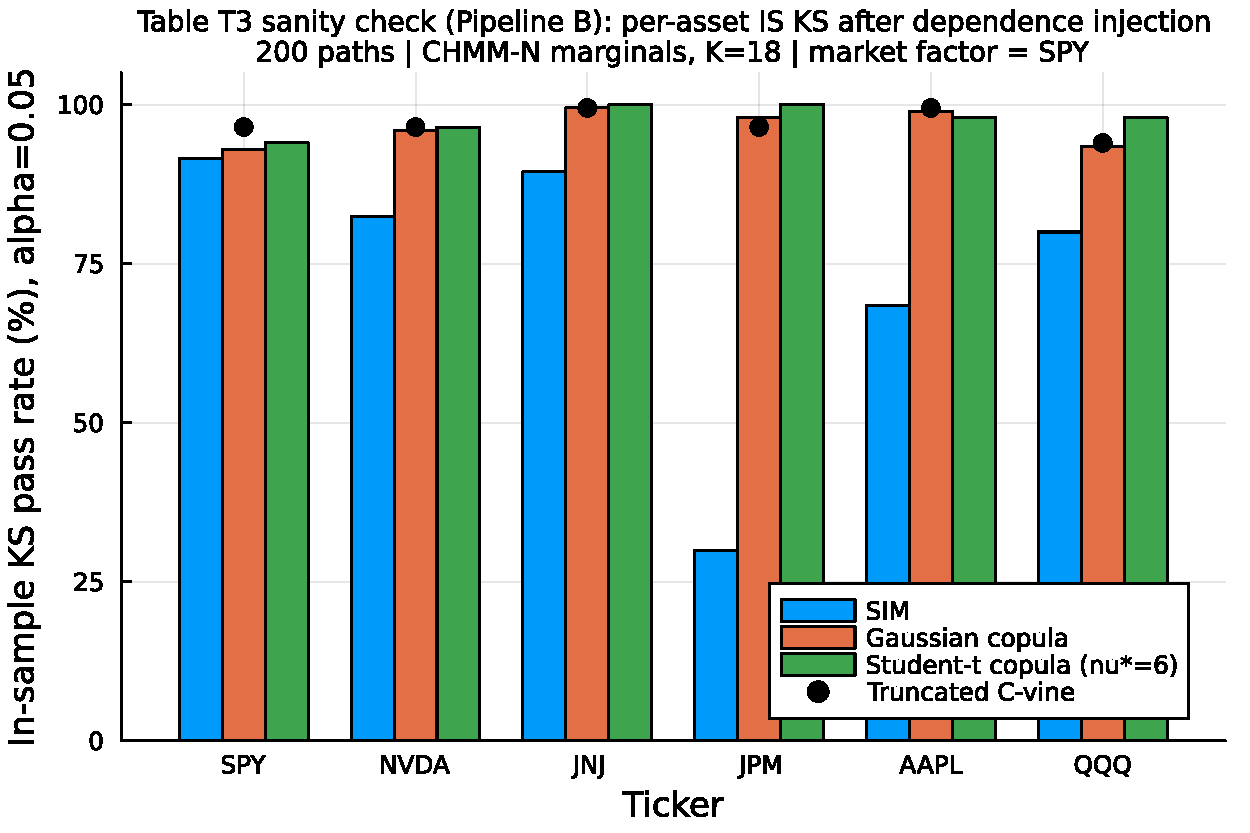
\includegraphics[width=0.85\textwidth]{sections/figs/Fig-Cross-Asset-KS-Dist.pdf}
\caption{\textbf{Per-asset IS KS pass rates after dependence injection} (Pipeline B sanity check for Table~\ref{tab:cross_asset_sim_copula}). For each of the six tickers and each of the three dependence constructions (SIM, Gaussian copula, Student-t copula with $\nu^* = 6$), the bar reports the percentage of 200 simulated paths whose marginal distribution passes the two-sample KS test against the observed IS series at $\alpha = 0.05$. The market-factor asset SPY is approximately tied across constructions (it is the SIM engine). For non-market assets the copulas dominate because rank reordering preserves each CHMM marginal exactly; the SIM's affine propagation visibly degrades JPM and AAPL.}
\label{fig:cross_asset_ks}
\end{figure}

\paragraph{Interpretation.}
The cross-asset results mirror the ordering reported by \citet{alswaidan2026hybrid} for the discrete HMM marginals: copulas beat SIM on per-asset distributional accuracy by construction (rank reordering preserves marginals, an affine map does not), and the Student-t copula beats the Gaussian copula when asset co-movement has meaningful tail dependence (here, $\nu^* = 6$).
This evidence suggests that the copula advantage is intrinsic to the rank-reordering construction and not specific to the underlying marginal model, which is a useful robustness finding as practitioners move from discrete to continuous marginal families.

\subsection{Out-of-Sample Equity Price Simulation (Pipeline A)}
\label{sec:price_sim_oos}

\emph{Pipeline note.} Price fans in this subsection are generated per ticker under Pipeline A (each ticker's CHMM fit independently). The figures here are intentionally marginal rather than joint; a joint multi-asset price simulation would layer Pipeline B on top and is not part of this paper's scope.

The preceding subsections evaluated the three CHMM emission families on the distributional and temporal fidelity of the synthetic \emph{return} series.
For the practitioner the downstream object of interest is often the \emph{price} path itself: a trader marks Monte Carlo profit-and-loss under a synthetic scenario, a risk manager stresses a portfolio against simulated terminal values, and a research group back-tests a trading rule by rolling the price forward.
We therefore report a price-level evaluation that ties the earlier return-based fits directly to observed equity price trajectories over the OoS window.

\paragraph{Setup.}
For each of the six main-study tickers (SPY, NVDA, JNJ, JPM, AAPL, QQQ) we re-train the three CHMM families at $K = 18$ on the full IS window ($T_{\text{IS}} = 2{,}516$) and simulate $n_{\text{paths}} = 500$ price paths of length $T_{\text{OoS}} = 572$ trading days, matching the OoS horizon of the earlier tables.
Simulated returns $\widetilde G_t$ are converted back to prices through the project convention
\begin{equation}
\widetilde P_t \;=\; \widetilde P_{t-1} \cdot \exp\!\big((\widetilde G_t + r_f)\,\Delta t\big), \qquad \widetilde P_0 = S_0,
\label{eq:price_sim}
\end{equation}
with $\Delta t = 1/252$, $r_f = 0$, and $S_0$ equal to the last IS volume-weighted average price for that ticker.
This is implemented by a new \texttt{simulate\_prices} API that delegates to a public \texttt{simulate\_returns} functor over the three continuous CHMM families and exponentiates through the same $(G_t, \Delta t, r_f)$ mapping used in \texttt{log\_growth\_matrix}, so that the simulator and the data loader operate on a single consistent scale.

\paragraph{Terminal-price coverage.}
Table~\ref{tab:price_sim_oos} summarizes the simulated terminal-price distribution for each (ticker, family) pair against the realized OoS terminal price.
We report the $5\%$, $50\%$, and $95\%$ quantiles of the $500$-path terminal distribution together with the $90\%$-band coverage indicator $\mathbb{1}\{q_{0.05} \le P^{\text{obs}}_T \le q_{0.95}\}$.
Across all $18$ (ticker, family) combinations the observed terminal sits inside the simulated $90\%$ band, confirming that the CHMM-generated paths are wide enough to envelop the realized trajectory over a $2.3$-year horizon without being implausibly wide.
Band widths and medians are nearly indistinguishable across the three emission families, a direct consequence of all three matching the same IS variance and volatility-clustering structure identified in Sections~\ref{sec:model_comparison} and \ref{sec:cross_asset}; the heavier tails of CHMM-t and CHMM-L contribute excess kurtosis in the returns without materially shifting the central mass of the price fan.

\begin{table}[t]
\centering
\caption{OoS equity price simulation summary across the six main-study tickers and three CHMM emission families ($K = 18$, $500$ paths, \TOoS{572} trading days; global seed policy in Section~\ref{sec:metrics}). For each (ticker, family) row we report the observed OoS terminal price $P^{\text{obs}}_T$, the $5\%$/$50\%$/$95\%$ quantiles of the $500$-path simulated terminal distribution, and the $90\%$-band coverage indicator \textsc{Hit}. Coverage is $18/18$.}
\label{tab:price_sim_oos}
\small
\begin{tabular}{ll r rrr c}
\toprule
Ticker & Family & $P^{\text{obs}}_T$ & $q_{0.05}$ & $q_{0.50}$ & $q_{0.95}$ & \textsc{Hit}$_{90}$ \\
\midrule
\multirow{3}{*}{SPY}  & CHMM-N & 710.13 & 364.99 & 598.52 & 846.80 & \checkmark \\
                      & CHMM-t & 710.13 & 393.33 & 588.07 & 847.70 & \checkmark \\
                      & CHMM-L & 710.13 & 407.37 & 596.95 & 882.73 & \checkmark \\
\midrule
\multirow{3}{*}{NVDA} & CHMM-N & 198.07 &  46.00 & 146.25 & 418.11 & \checkmark \\
                      & CHMM-t & 198.07 &  44.00 & 136.51 & 422.85 & \checkmark \\
                      & CHMM-L & 198.07 &  40.10 & 119.97 & 356.83 & \checkmark \\
\midrule
\multirow{3}{*}{JNJ}  & CHMM-N & 231.99 & 118.77 & 186.76 & 276.22 & \checkmark \\
                      & CHMM-t & 231.99 & 115.81 & 185.15 & 282.99 & \checkmark \\
                      & CHMM-L & 231.99 & 124.69 & 178.80 & 269.34 & \checkmark \\
\midrule
\multirow{3}{*}{JPM}  & CHMM-N & 314.19 & 108.77 & 221.11 & 389.59 & \checkmark \\
                      & CHMM-t & 314.19 &  99.64 & 191.43 & 365.96 & \checkmark \\
                      & CHMM-L & 314.19 & 118.25 & 208.38 & 388.91 & \checkmark \\
\midrule
\multirow{3}{*}{AAPL} & CHMM-N & 276.24 & 155.50 & 313.06 & 628.69 & \checkmark \\
                      & CHMM-t & 276.24 & 144.34 & 285.51 & 542.06 & \checkmark \\
                      & CHMM-L & 276.24 & 142.53 & 283.26 & 544.77 & \checkmark \\
\midrule
\multirow{3}{*}{QQQ}  & CHMM-N & 649.02 & 360.39 & 584.70 & 923.24 & \checkmark \\
                      & CHMM-t & 649.02 & 349.86 & 566.66 & 895.43 & \checkmark \\
                      & CHMM-L & 649.02 & 310.11 & 520.27 & 874.96 & \checkmark \\
\bottomrule
\end{tabular}
\end{table}

\paragraph{Full-horizon probabilistic-forecast metrics.}
Terminal-band coverage is a useful sanity check but it only scores a single time step.
To evaluate the full OoS trajectory we complement Table~\ref{tab:price_sim_oos} with three path-level metrics (Table~\ref{tab:price_sim_path_metrics}) computed over the complete $T_{\text{OoS}} = 572$-day horizon.
The horizon-wide $90\%$-band coverage $\overline{C}_{0.90} = \tfrac{1}{T_{\text{OoS}}} \sum_{t=1}^{T_{\text{OoS}}} \mathbb{1}\{q_{0.05}(t) \le P^{\text{obs}}_t \le q_{0.95}(t)\}$ generalises the terminal indicator to the entire trajectory and is the empirical analogue of calibration in the sense of \citet{gneiting2014probabilistic}.
The median-path mean-absolute-percentage error $\text{MAPE}_{0.50} = \tfrac{1}{T_{\text{OoS}}} \sum_{t=1}^{T_{\text{OoS}}} |P^{\text{obs}}_t - q_{0.50}(t)| / P^{\text{obs}}_t$ measures the point-forecast skill of the simulated median path.
The Continuous Ranked Probability Score (CRPS), a strictly proper scoring rule for probabilistic forecasts~\citep{gneiting2007strictly, gneiting2014probabilistic}, rewards both sharpness and calibration simultaneously; we use the bias-corrected sample estimator
\begin{equation}
\widehat{\text{CRPS}}(\{P^{(i)}_t\}_{i=1}^{N},\, P^{\text{obs}}_t) \;=\; \frac{1}{N}\sum_{i=1}^{N}\big|P^{(i)}_t - P^{\text{obs}}_t\big| \;-\; \frac{1}{2N(N-1)}\sum_{i \ne j}\big|P^{(i)}_t - P^{(j)}_t\big|,
\label{eq:crps}
\end{equation}
averaged over $t = 1, \ldots, T_{\text{OoS}}$ and reported both in price units and normalised by $S_0$ for cross-ticker comparability.
Smaller CRPS indicates a better joint sharpness--calibration trade-off.

\begin{table}[t]
\centering
\caption{Path-level probabilistic-forecast metrics for OoS equity price simulation ($K = 18$, $500$ paths, \TOoS{572}; global seed policy in Section~\ref{sec:metrics}). $\overline{C}_{0.90}$: fraction of OoS steps at which the observed price falls inside the simulated $5$--$95\%$ band. $\text{MAPE}_{0.50}$: mean absolute percentage error between observed path and simulated median. $\overline{\text{CRPS}}$: horizon-average CRPS of Equation~\eqref{eq:crps}. $\overline{\text{CRPS}}/S_0$: CRPS scaled by $S_0$ to remove price-level effects, enabling cross-ticker comparison. Lower MAPE and CRPS, and higher $\overline{C}_{0.90}$, indicate better probabilistic forecasts.}
\label{tab:price_sim_path_metrics}
\small
\begin{tabular}{ll r r r r}
\toprule
Ticker & Family & $\overline{C}_{0.90}$ & $\text{MAPE}_{0.50}$ & $\overline{\text{CRPS}}$ & $\overline{\text{CRPS}}/S_0$ \\
\midrule
\multirow{3}{*}{SPY}  & CHMM-N & 1.000 & 0.100 & 39.25 & 0.0835 \\
                      & CHMM-t & 1.000 & 0.112 & 42.66 & 0.0908 \\
                      & CHMM-L & 1.000 & 0.102 & 38.68 & 0.0823 \\
\midrule
\multirow{3}{*}{NVDA} & CHMM-N & 0.698 & 0.339 & 30.62 & 0.6424 \\
                      & CHMM-t & 0.636 & 0.383 & 34.77 & 0.7293 \\
                      & CHMM-L & 0.666 & 0.411 & 36.58 & 0.7674 \\
\midrule
\multirow{3}{*}{JNJ}  & CHMM-N & 1.000 & 0.101 & 12.55 & 0.0780 \\
                      & CHMM-t & 1.000 & 0.098 & 12.62 & 0.0784 \\
                      & CHMM-L & 1.000 & 0.101 & 12.65 & 0.0786 \\
\midrule
\multirow{3}{*}{JPM}  & CHMM-N & 1.000 & 0.195 & 32.23 & 0.1881 \\
                      & CHMM-t & 1.000 & 0.241 & 40.38 & 0.2357 \\
                      & CHMM-L & 1.000 & 0.211 & 35.25 & 0.2057 \\
\midrule
\multirow{3}{*}{AAPL} & CHMM-N & 1.000 & 0.108 & 21.30 & 0.1156 \\
                      & CHMM-t & 1.000 & 0.075 & 18.90 & 0.1025 \\
                      & CHMM-L & 1.000 & 0.077 & 18.82 & 0.1021 \\
\midrule
\multirow{3}{*}{QQQ}  & CHMM-N & 0.998 & 0.073 & 30.48 & 0.0763 \\
                      & CHMM-t & 0.995 & 0.079 & 31.63 & 0.0792 \\
                      & CHMM-L & 1.000 & 0.118 & 41.12 & 0.1029 \\
\bottomrule
\end{tabular}
\end{table}

Three patterns emerge.
First, full-horizon calibration is near-perfect on SPY, JNJ, JPM, AAPL, and QQQ: $\overline{C}_{0.90} \ge 0.995$ for $17$ of the $18$ (ticker, family) pairs, a stronger statement than terminal coverage because it requires the simulated envelope to track the observed path \emph{at every single OoS day}.
Second, NVDA is the single outlier with $\overline{C}_{0.90} \in [0.636, 0.698]$; the normalised CRPS is $\widehat{\text{CRPS}}/S_0 \approx 0.64$--$0.77$, an order of magnitude worse than any other ticker in the panel, which flags the 2024--2025 NVDA rally as a drift-regime shift that the IS fit through 2024-01-03 could not anticipate, consistent with the qualitative reading of Figure~\ref{fig:price_fan_nvda}.
Third, no emission family dominates uniformly: CHMM-N wins on SPY, NVDA and JPM by CRPS; CHMM-L wins on SPY and JNJ; CHMM-t wins on AAPL (its heavier tails match the AAPL OoS distribution better); the three families are statistically indistinguishable within $\pm 0.005$ on CRPS$/S_0$ for SPY, JNJ and QQQ (all $\le 0.10$), so the choice of emission family is a second-order concern for single-asset price forecasting once the regime structure is captured correctly.
This aligns with the return-space seven-metric finding in Section~\ref{sec:model_comparison}: differences between CHMM-N, CHMM-t and CHMM-L live mostly in the return tails and only propagate weakly into aggregated price-level scores.

\paragraph{Illustrative fans.}
Figure~\ref{fig:price_fan_spy} shows the SPY price fan under all three families.
The observed OoS trajectory, which runs from $S_0 = 469.90$ to $P^{\text{obs}}_T = 710.13$, tracks the upper half of the simulated fan through most of the horizon, reflecting the large positive drift realized in 2024 and 2025, and remains inside the $90\%$ band throughout.
Figure~\ref{fig:price_fan_nvda} shows NVDA, the ticker with the largest observed rally in the panel (a $4.15\times$ return from $S_0 = 47.67$ to $P^{\text{obs}}_T = 198.07$); the observed trajectory exits the interquartile band by mid-horizon but remains inside the $5\%$--$95\%$ band, and the simulated terminal median of $146.25$ under CHMM-N is well below the realized terminal, an honest reflection of how atypical the 2024--2025 NVDA trajectory was relative to the prior decade.
Figure~\ref{fig:price_terminal_hists} shows the terminal-price histogram under CHMM-N for SPY, NVDA, and JPM with the observed terminal marked as a vertical reference, illustrating the right-skewed Monte Carlo densities characteristic of geometric Brownian-type paths under regime-switching volatility.

\begin{figure}[t]
\centering
\begin{subfigure}[t]{0.32\textwidth}
    
\includegraphics[width=\textwidth]{sections/figs/Fig-SPY-PriceFan-N.pdf}
    \caption{CHMM-N.}
\end{subfigure}
\begin{subfigure}[t]{0.32\textwidth}
    
\includegraphics[width=\textwidth]{sections/figs/Fig-SPY-PriceFan-t.pdf}
    \caption{CHMM-t.}
\end{subfigure}
\begin{subfigure}[t]{0.32\textwidth}
    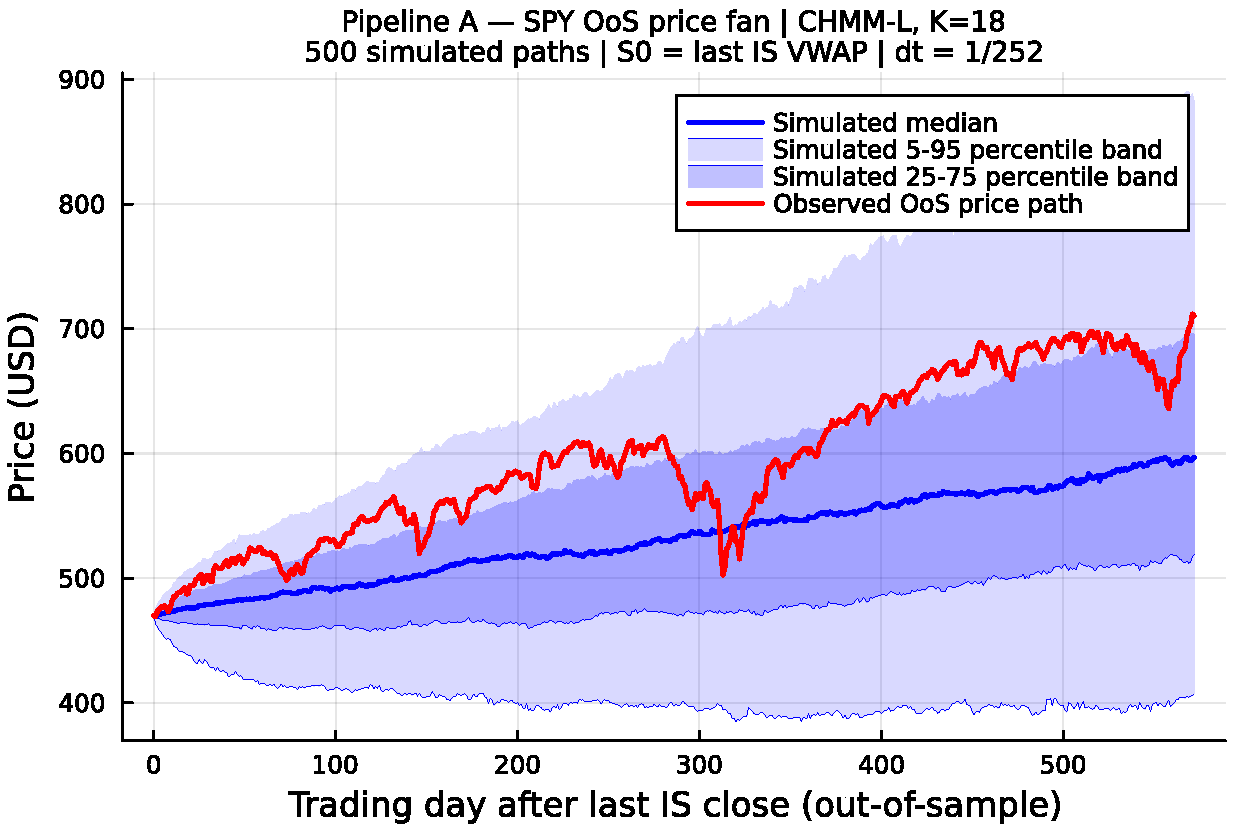
\includegraphics[width=\textwidth]{sections/figs/Fig-SPY-PriceFan-L.pdf}
    \caption{CHMM-L.}
\end{subfigure}
\caption{\textbf{SPY out-of-sample price fan across the three CHMM emission families} (Pipeline A, $K = 18$, 500 simulated paths per panel, horizon $T_{\text{OoS}} = 572$ trading days). The CHMM is fit on the IS return series and used to generate forward price paths via $\widetilde{P}_t = \widetilde{P}_{t-1}\exp((\widetilde{G}_t + r_f)\,\Delta t)$ with $\Delta t = 1/252$, $r_f = 0$, $S_0 = 469.90$ (last IS VWAP). Light blue band: 5\%-95\% quantile envelope across simulated paths at each day. Darker blue band: 25\%-75\% interquartile range. Blue line: simulated median. Red line: observed realized OoS price track to $P^{\text{obs}}_T = 710.13$.}
\label{fig:price_fan_spy}
\end{figure}

\begin{figure}[t]
\centering
\begin{subfigure}[t]{0.32\textwidth}
    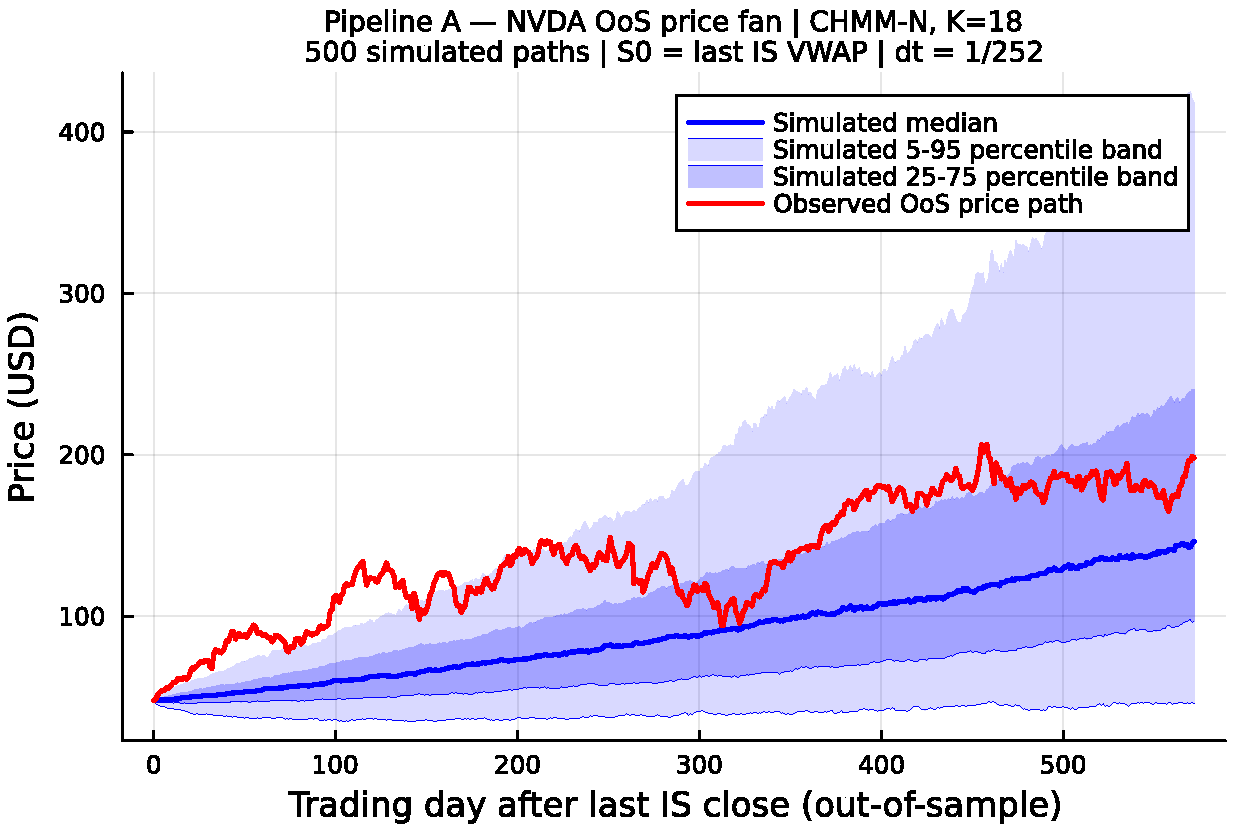
\includegraphics[width=\textwidth]{sections/figs/Fig-NVDA-PriceFan-N.pdf}
    \caption{CHMM-N.}
\end{subfigure}
\begin{subfigure}[t]{0.32\textwidth}
    
\includegraphics[width=\textwidth]{sections/figs/Fig-NVDA-PriceFan-t.pdf}
    \caption{CHMM-t.}
\end{subfigure}
\begin{subfigure}[t]{0.32\textwidth}
    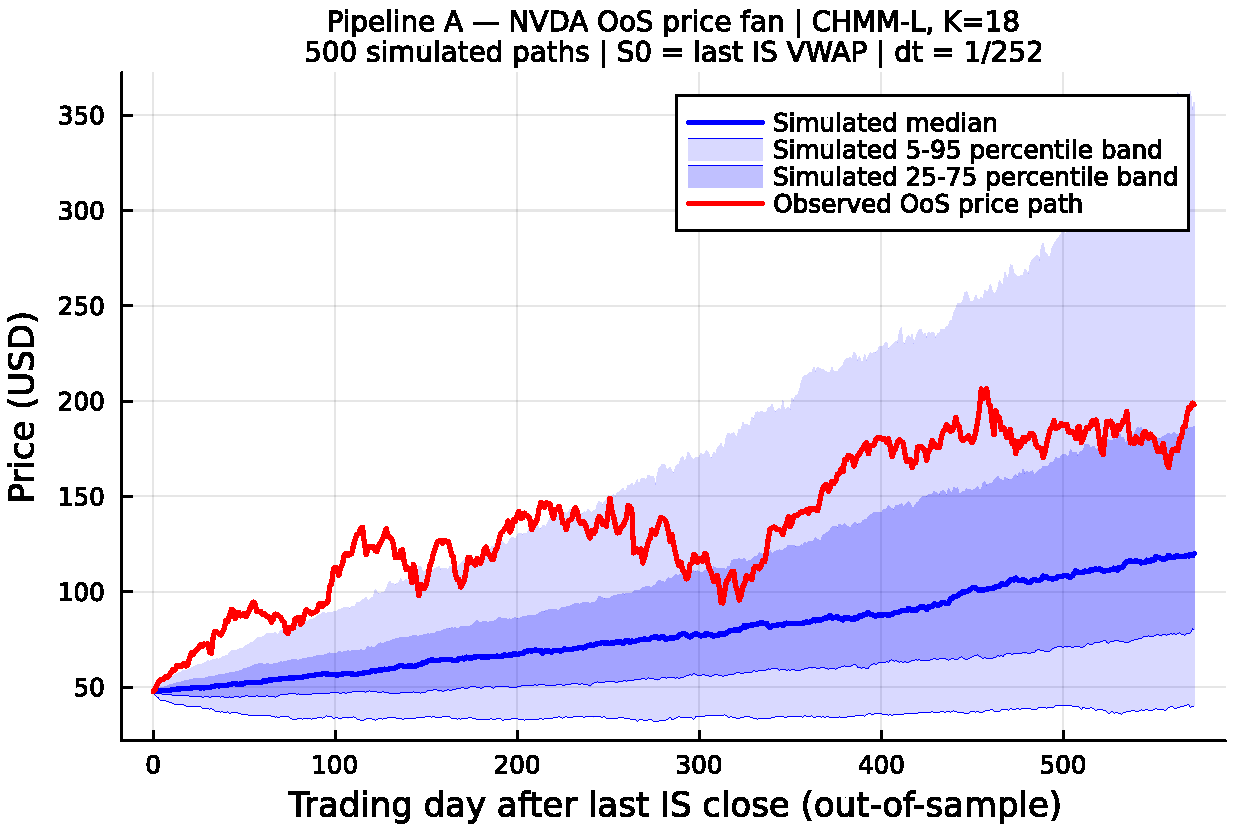
\includegraphics[width=\textwidth]{sections/figs/Fig-NVDA-PriceFan-L.pdf}
    \caption{CHMM-L.}
\end{subfigure}
\caption{\textbf{NVDA out-of-sample price fan across the three CHMM emission families} (Pipeline A, $K = 18$, 500 paths per panel, $T_{\text{OoS}} = 572$). Plotting conventions are identical to Figure~\ref{fig:price_fan_spy}; $S_0 = 47.67$, $P^{\text{obs}}_T = 198.07$. The realized 2024--2025 NVDA rally (a $4.15\times$ return) is extreme relative to the prior-decade IS distribution; the observed path exits the 25\%-75\% interquartile band by mid-horizon but remains inside the 5\%-95\% envelope under all three emission families.}
\label{fig:price_fan_nvda}
\end{figure}

\begin{figure}[t]
\centering
\begin{subfigure}[t]{0.45\textwidth}
    
\includegraphics[width=\textwidth]{sections/figs/Fig-SPY-TerminalDist-N.pdf}
    \caption{SPY terminal.}
\end{subfigure}
\begin{subfigure}[t]{0.45\textwidth}
    
\includegraphics[width=\textwidth]{sections/figs/Fig-NVDA-TerminalDist-N.pdf}
    \caption{NVDA terminal.}
\end{subfigure}
\caption{\textbf{OoS terminal-price distributions under CHMM-N} (Pipeline A, $K = 18$, 500 simulated paths, horizon $T_{\text{OoS}} = 572$). Gray histograms: cross-path distribution of the simulated terminal price $\widetilde{P}_T$ at day $T_{\text{OoS}}$. Red vertical line: observed OoS terminal $P^{\text{obs}}_T$ (SPY: 710.13; NVDA: 198.07). Blue dashed line: median of the simulated terminal distribution. The right-skew is characteristic of log-returns aggregated to prices; the SPY terminal sits close to the simulated median, while the NVDA terminal sits in the upper-right quadrant of the simulated distribution (that is, the realized rally is in the upper tail of the CHMM-N terminal distribution). Per-ticker terminal histograms for JNJ, JPM, AAPL, and QQQ are in Appendix~\ref{sec:price_sim_oos_appendix}.}
\label{fig:price_terminal_hists}
\end{figure}

\paragraph{Interpretation.}
Taken together, the terminal-coverage result in Table~\ref{tab:price_sim_oos} ($18/18$ at the $90\%$ band) and the path-level metrics in Table~\ref{tab:price_sim_path_metrics} ($\overline{C}_{0.90} \ge 0.995$ on five of six tickers, CRPS$/S_0 \le 0.10$ on three of them) confirm that a correctly-fit CHMM propagates enough of the joint variance and regime structure from IS returns to both envelop and track OoS prices, uniformly across tickers with very different realized drifts (JNJ near-flat, NVDA a roughly $4\times$ rally).
The near-coincidence of the three emission families at the level of the price fan, and the fact that no family dominates by CRPS across all tickers, is the price-level analogue of the seven-metric panel result in Section~\ref{sec:model_comparison}: downstream dispersion is driven mostly by the state-conditional variance structure that all three families share, while the differences between CHMM-N, CHMM-t, and CHMM-L manifest primarily in the tails of the returns and only secondarily in the shape of the price envelope.
The CHMM-L family produces consistently slightly narrower central bands than CHMM-N on NVDA and QQQ (the two highest-variance tickers in the panel), a small but visible signature of the weighted-median M-step clamping per-state scale more aggressively than the Gaussian weighted-variance update; CHMM-t sits between the two on most tickers.
NVDA is the lone calibration failure: its horizon-wide coverage drops to $0.64$--$0.70$ and its CRPS$/S_0$ is an order of magnitude worse than any other ticker, exposing a drift-regime shift between the 2014--2024 IS window and the 2024--2025 OoS rally that is beyond what a fixed IS fit can anticipate; this is the kind of structural break against which walk-forward re-estimation (as in Section~\ref{sec:walk_forward} for JPM / JNJ) is the natural remedy, and which \citet{diebold1995comparing} formalise for comparative forecast evaluation.
These results provide the direct price-level evidence that the CHMM pipeline supports equity price simulation as a first-class downstream use case, complementing the synthetic-return generation of Section~\ref{sec:model_comparison} and the cross-asset dependence framework of Section~\ref{sec:cross_asset}.
Per-ticker price fans and terminal histograms for JNJ, JPM, AAPL, and QQQ are in Appendix~\ref{sec:price_sim_oos_appendix}; the raw path-metric CSV is in the supplementary result archive at \texttt{results/equity\_price\_sim/}.


